\documentclass[11pt]{article} % use larger type; default would be 10pt
\usepackage[utf8]{inputenc} % set input encoding (not needed with XeLaTeX)

\usepackage[ngerman]{babel}% deutsche Trennregeln
\usepackage[T1]{fontenc}% wichtig für Trennung von Wörtern mit Umlauten
\usepackage{lmodern}

%%% PAGE DIMENSIONS
\usepackage{geometry} % to change the page dimensions
\geometry{a4paper, left=30mm, right=40mm, top=25mm, bottom=20mm}

%Listen
\usepackage{enumitem} 

\usepackage{cite}
%%%%%%%%%%%%%%%%%%
% Mathe Packages %
%%%%%%%%%%%%%%%%%%

\usepackage{amsmath}
\usepackage{amsthm}
\usepackage{amssymb}
\usepackage{mathtools}
\usepackage{bbm}


%Links
\usepackage{hyperref}
\hypersetup{
    colorlinks,
    citecolor=black,
    filecolor=black,
    linkcolor=black,
    urlcolor=black
}


%%%%%%%%%%%%%%%%%%%%%%%%%
% Mathematische Symbole %
%%%%%%%%%%%%%%%%%%%%%%%%%

%Topologie
\newcommand{\Borel}{\mathcal{B}}

%masstheorie
\newcommand{\ind}{\mathbbm{1}}

\newcommand{\N}{\mathbb{N}}
\newcommand{\Z}{\mathbb{Z}}
\newcommand{\Zp}{{\Z_p}}
\newcommand{\R}{\mathbb{R}}
\newcommand{\C}{\mathbb{C}}
\newcommand{\Q}{\mathbb{Q}}
\newcommand{\A}{\mathbb{A}}
\newcommand{\I}{\mathbb{I}}
\newcommand{\K}{\Q}
\newcommand{\Sw}{S}
\newcommand{\Aq}{\A_\Q}
\newcommand{\Ak}{\A_\K}
\newcommand{\Iq}{\I_\Q}
\newcommand{\kinf}{\K_\infty}
\newcommand{\Kp}{{\K_p}}
\newcommand{\ginf}{g_\infty}
\newcommand{\tinf}{t_\infty}
\newcommand{\finf}{f_\infty}
\newcommand{\xinf}{x_\infty}
\newcommand{\xiinf}{\xi_\infty}
\newcommand{\finft}{\hat{f}_\infty}



\newcommand{\rdprod}[1]{\prod\limits_{#1}'}{%{\widehat{\prod\limits_{#1}}}

\DeclarePairedDelimiter\abso{\lvert}{\rvert}

% Swap the definition of \abs* and \norm*, so that \abs
% and \norm resizes the size of the brackets, and the 
% starred version does not.
\makeatletter
\let\oldabs\abso
\def\abso{\@ifstar{\oldabs}{\oldabs*}}

\newcommand{\abs}[1][\,\cdot\,]{\abso{#1}}

\newcommand{\highlight}[1]{\textit{#1}}

%%%%%%%%%%%%
% Theoreme %
%%%%%%%%%%%%



\theoremstyle{definition}
\newtheorem{defi}{Definition}[section]
\newtheorem{bsp}[defi]{Beispiele}

\theoremstyle{plain}
\newtheorem{satz}[defi]{Satz}
\newtheorem{proposition}[defi]{Satz}
\newtheorem{lemma}[defi]{Lemma}



\begin{document}

\pagenumbering{Roman}

%%%Deckblatt
%

%%% Inhaltsverzeichnis
\tableofcontents
\clearpage

\pagenumbering{arabic}   



%%%%%%%%%%%%%%%%%%%Beginn
\section{Die Hausarbeit in der Praxis}
\label{sec:kapitel2}




Hier steht ein kurzer einleitender Text zwischen den beiden Überschriften.



\subsection{Die Quellenverwaltung und Zitiertechnik}
Für die Quellenverwaltung empfehlen wir die Software Citavi, welche unter folgendem Link kostenlos zu beziehen ist: \underline{http://citavi.com/de/download.html}\\
Als Zitationsstil ist der Citavi Basis-Stil (deutsch) zu werden, was den Grundeinstellungen entspricht (bzw. Citavi Default Style (englisch)).
\begin{figure}[!htb]
\centering
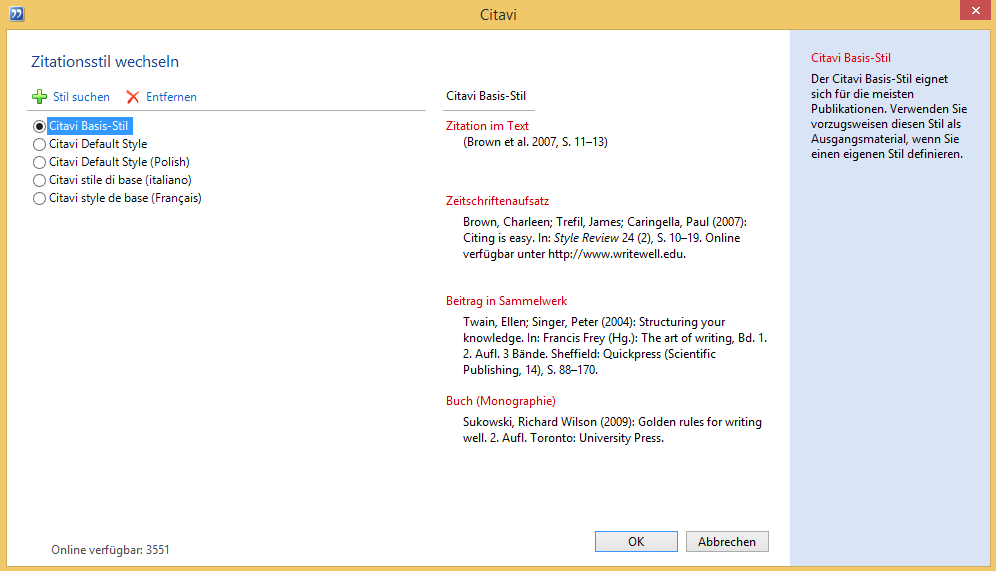
\includegraphics[scale=0.45]{Bilder/Citavi.png}
\end{figure}

Zitate sind grundsätzlich in den Fließtext einzufügen. Fußnoten werden für Zitate nicht genutzt. Nur wenn eine Einbindung der Information in den Text nicht möglich oder sinnvoll ist, kann eine Fußnote genutzt werden. Direkte Zitate sollten vermieden, stattdessen indirekte Zitate bevorzugt werden. Inhalte von Fußnoten sollten möglichst in den Text eingearbeitet werden.
$\;$\\
\begin{spacing}{1}
\textbf{Beitrag in einem Sammelband}\\

Beispiel Literaturangabe:\\

Degele, Nina (2005): Neue Kompetenzen im Internet. In: Kai Lehmann und Michael Schetsche (Hg.): Die Google-Gesellschaft. Wissen im 21. Jahrhundert. Bielefeld: transcript, S. 63–74. \\

\textbf{Buch (Monographie)}\\

Beispiel Literaturangabe:\\

Andretta, Susie; Dervall, John; Li, Han (2005): Information literacy. A practitioner's guide. Oxford: Chandos (Chandos information professionals series). \\

\textbf{Hochschulschrift}\\

Beispiel Literaturangabe:\\

Zweifel, Aron (2005): Information Literacy Konzeption eines Teaching Library-Moduls am Beispiel der Fachhochschulbibliothek Frankfurt am Main. Diplomarbeit. Fachhochschule Frankfurt a. M., Frankfurt a.M. Online verfügbar unter\\ www.fh-frankfurt.de/de/.media/bibliothek/aronzweifel-ilkonzeption-tlmoduls-fh-ffm.pdf, zuletzt geprüft am 30.01.2009.\\

\textbf{Internetdokument}\\

Beispiel Literaturangabe:\\

Arbeitsgemeinschaft Informationskompetenz NRW (2005): ULB Bonn - AG Informationskompetenz - Schulungs- und Lernmaterialien. Online verfügbar unter\\ www.informationskompetenz.de, zuletzt aktualisiert am 24.04.2005, zuletzt geprüft am\\ 30.01.2009.\\
\end{spacing}

Internetzitate werden analog zu den direkten und indirekten Zitaten genutzt. Eine Internetquelle ist nur dann zu zitieren, wenn ein Autor und ein Erscheinungsjahr für die Quelle verfügbar sind.\\

\begin{spacing}{1}

\textbf{Zeitschriftenaufsatz}\\

Beispiel Literaturangabe:\\

Correia, Ana Maria Ramalho; Teixeira, José Carlos (2003): Information literacy. An integrated concept for a safer Internet. In: Online Information Review 27 (5), S. 311–320.\\

\textbf{Zitation im Text:}\\

Beispiele:\\

Ein Autor: (Degele 2005, S. 63)\\
Zwei Autoren: (Correia und Teixeira 2003, S. 319)\\
Ab drei Autoren: (Andretta et al. 2005, S. 5)\\

\end{spacing}

Jedes Werk, aus dem zitiert wurde, muss im Literaturverzeichnis aufgeführt werden. Werke, die zur Erarbeitung des Themas genutzt aber nicht zitiert wurden, gehören nicht ins Literaturverzeichnis. \\

Die Universitätsbibliothek bietet Ihnen mit dem Literaturverwaltungsprogramm RefWorks ebenso ein persönliches und kostenfreies Tool für die professionelle Verwaltung Ihrer Literaturangaben. Weitere Informationen finden sich auf der Uni-Homepage:\\http://www.bibliothek.uni-augsburg.de/service/literaturverwaltung/refworks/









\clearpage


\subsection{Der Schreib- und Forschungsprozess}

\begin{figure}[h]
\centering
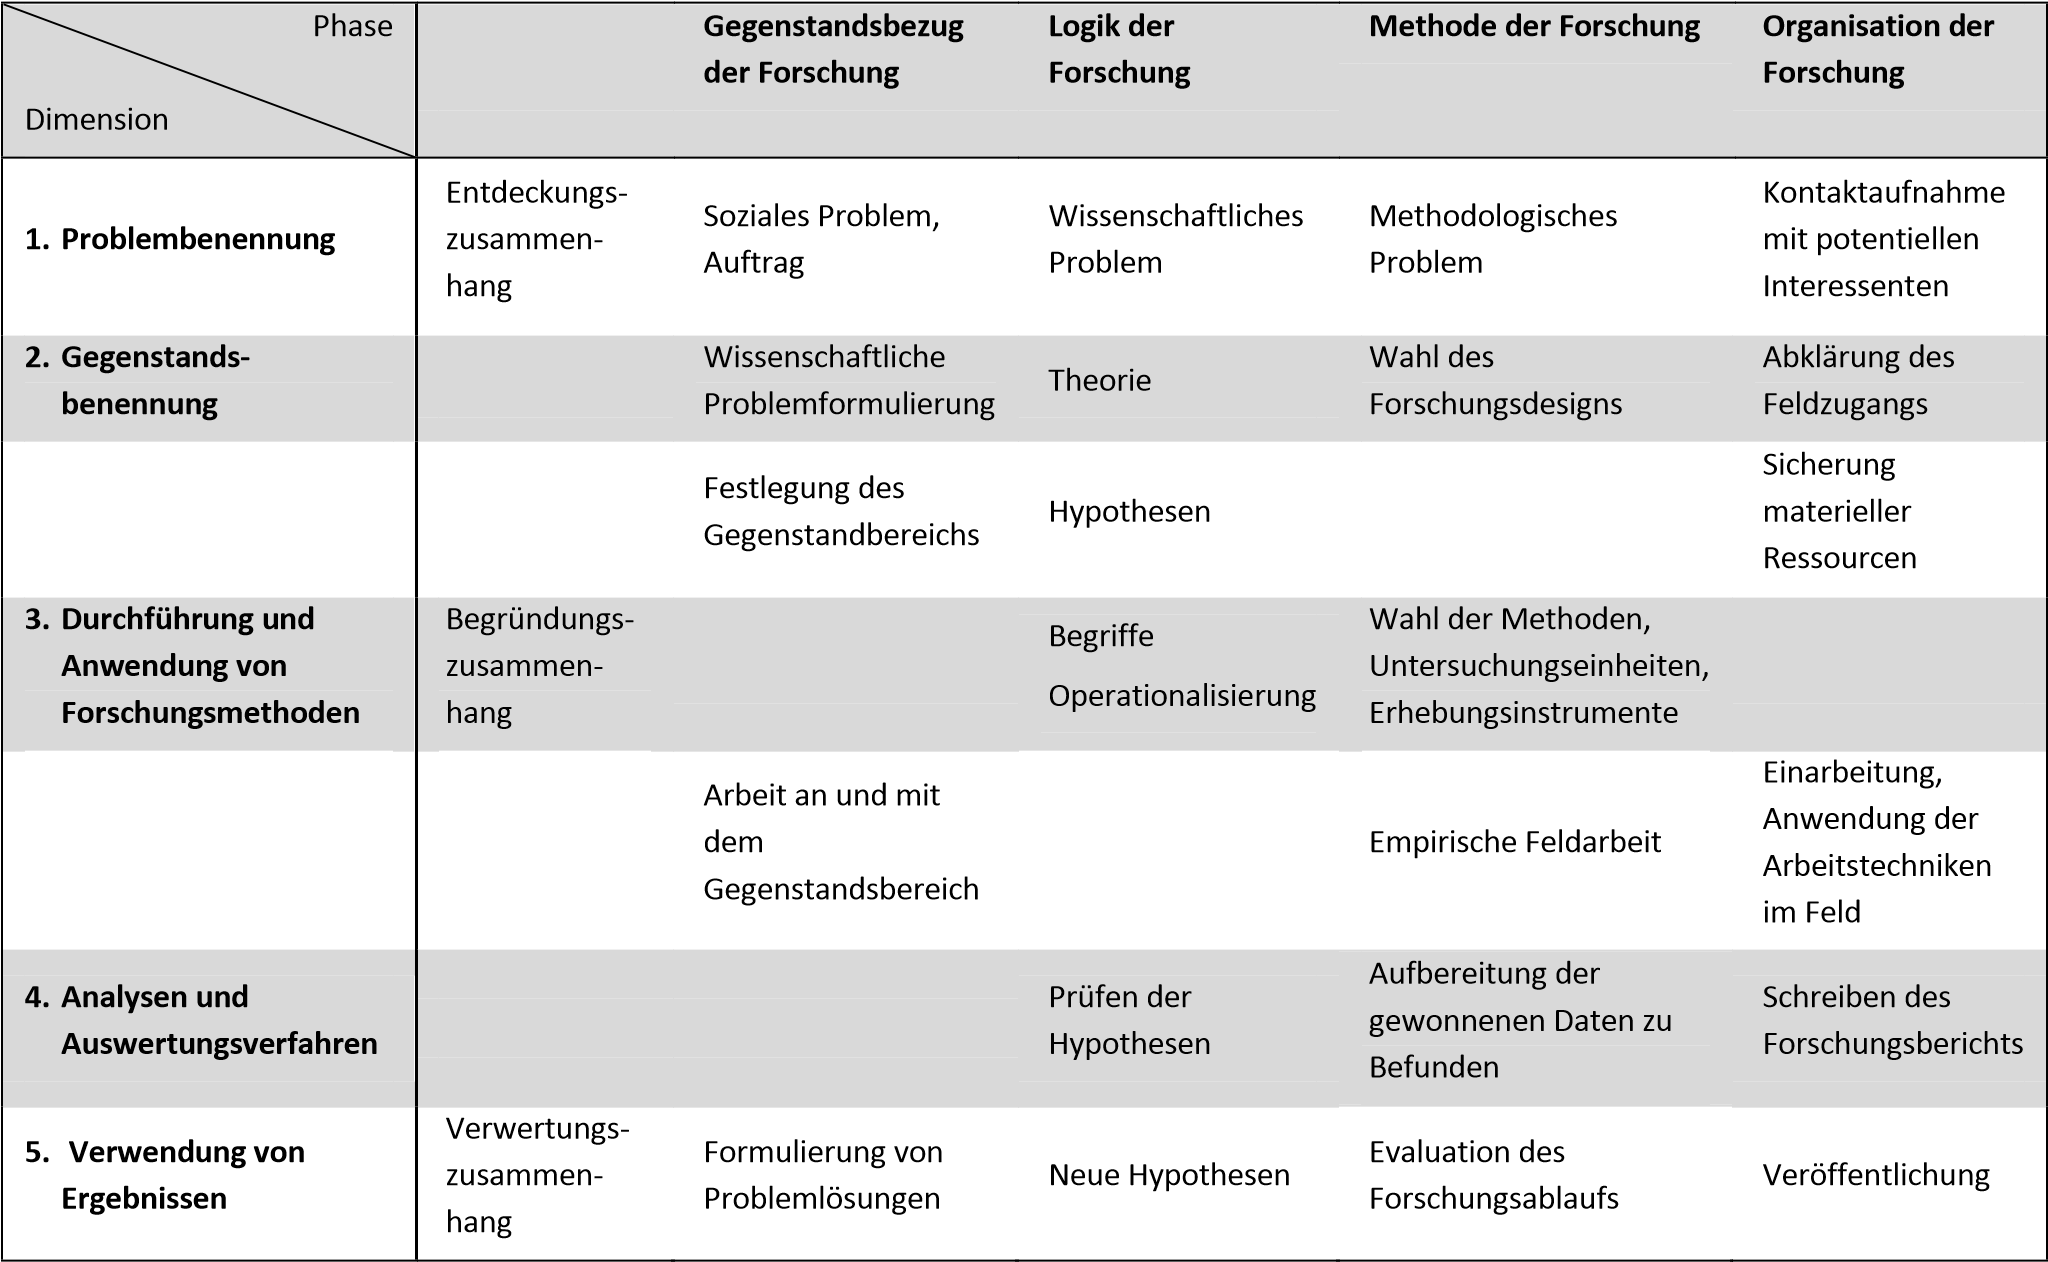
\includegraphics[width=1\textwidth]{Bilder/Abbildung.png}
Quelle: \citet{atteslander2010}, S. 13
\caption{Dimension einer wissenschaftlichen Arbeit nach Peter Atteslander}
\label{abb:abbildung1}
\end{figure}










\clearpage



\subsection{Bestandteile einer wissenschaftlichen Arbeit}


\begin{table}[htbp]
\renewcommand{\arraystretch}{1.4} 
  \centering

    \begin{tabular}{|l|l|}
\hline
    \textbf{{\large Hauptgruppe}} &  \textbf{{\large Bestandteile}} \\  \hline
    Titel &  $\cdot \quad$ Titelblatt \\ \hline
    Einleitungsapparat &  $\cdot \quad$ Abstract \\
	& $\cdot \quad$ Inhaltsverzeichnis \\
          &  $\cdot \quad$ Abbildungsverzeichnis \\
          &  $\cdot \quad$ Tabellenverzeichnis \\
	&  $\cdot \quad$ Abkürzungsverzeichnis \\ \hline
    Einführung &  $\cdot \quad$ Kurze Hinführung zum Thema \\ \hline
    Hauptteil &  $\cdot \quad$ Detaillierte Behandlung des Themas  \\ \hline
    Schluss &  $\cdot \quad$ Zusammenfassung und Ausblick \\ \hline
    Abschlussapparat & $\cdot \quad$ Anhang \\
	& $\cdot \quad$ Literaturverzeichnis \\
          &  $\cdot \quad$ Eidesstattliche Erklärung \\ \hline

    \end{tabular}%
  \label{tab:tabelle1}%



$\;$\\

\caption{Bestandteile einer wissenschaftlichen Hausarbeit}

Quelle: \citet{atteslander2010}, S. 13

\end{table}
Tabellen und Abbildungen unterstreichen Aussagen und illustrieren Forschungsergebnisse, um deren Verständnis für den Leser zu erleichtern. Sie dürfen nur dann eingesetzt werden, wenn sie im Text ausführlich erläutert werden. Bitte achten Sie darauf, dass die Tabellen selbsterklärend und notwendige Inhalte in die Tabellenbeschreibung aufzunehmen sind. Qualitativ müssen alle Abbildungen und Tabellen so hochwertig sein, dass sie sowohl auf dem Bildschirm, als auch auf einem Ausdruck klar und deutlich lesbar sind. Formal benötigt jede Abbildung eine Abbildungsunterschrift, jede Tabelle eine Tabellenüberschrift. Außerdem ist jeweils eine Quellenangabe, entsprechend der Zitation im Text, anzufügen.\\
Stilistisch ist auf eine neutrale Formulierung zu achten. Formulierungen mit „ich, man, wir, es“ sollten unbedingt vermieden werden.







\clearpage

\section{Harmonische Analysis}

\subsection{Lokalkompakte Gruppen}
%topologische Gruppe: done
%charaktere:partly
%haar masse: done
%fouriertransformation:done
%pontryagin erwaehnen: done
Am Anfang steht immer eine
\begin{defi}
	Eine \highlight{topologische Gruppe} ist eine Gruppe $G$ zusammen mit einer Topologie, welche die folgenden Eigenschaften erf"ullt:
		\begin{enumerate}[label=(\roman*)] % leftmargin=*, align=left, labelsep=1pt]
			\item Die Gruppenoperation
				\begin{align*}
					G \times G &\longrightarrow G\\
					(g,h) &\longmapsto gh
				\end{align*}
			stetig auf der Produkttopologie von $G \times G$.
			\item Die Umkehrabbildung
				\begin{align*}
					G &\longrightarrow G\\
					g &\longmapsto g^{-1}
				\end{align*}
				ist stetig.
		\end{enumerate}
	Ein \emph{Homomorphismus topologischer Gruppen} $G_1$ und $G_2$ ist eine stetiger Gruppenhomomorphismus $G_1 \to G_2$.
	Ist dieser bijektiv und die Umkehrabbildung wieder ein Homomorphismus topologischer Gruppen, so sprechen wir von einem \emph{Isomorphismus topologischer Gruppen}.
\end{defi}
	
	Man sieht sofort, dass die Translationen um ein beliebiges Gruppenelement ein Homeomorphismus $G \to G$ bilden.
	Die Topologie ist also \emph{translationsinvariant} in dem Sinne, dass f"ur alle $g \in G$ und jede Mengen $U$ die "Aquivalenzen
	\begin{align*}
		U \text{ ist offen} \Leftrightarrow gU = \{gu \in G: u\in U\} \text{ ist offen} \Leftrightarrow Ug = \{ug \in G: u\in U\} \text{ ist offen}
	\end{align*}
	gelten.
	Analog verh"alt es sich f"ur die Umkehrabbildung. Sie ist ein Homeomorphismus und $U$ ist genau dann offen, wenn $U^{-1}=\{u^{-1}\in G: u \in U\}$ offen ist.
	
	Die Translationsinvarianz der Topologie hat nun einige nette Vorteile.
	Zum Beispiel wird bereits die ganze Topologie durch die Umgebungsbasis des neutralen Elements definiert.
	Durch Translation erhalten wir Umgebungsbasen beliebiger anderer Elemente und damit zwangsl"aufig die komplette Topologie.
	F"ur ein weiteres Beispiel erinnern wir uns an die Definition der Stetigkeit in topologischen R"aumen.
	Eine Abbildung $f: G_1 \to G_2$ zwischen zweier topologischer R"aume heißt stetig, wenn f"ur alle $g\in G_1$ und jede offene Umgebung $U$ von $f(g)$ eine offene Umgebung $V$ von $g$ existiert, sodass $f(V)\subseteq U$.
	Sind $G_1$ und $G_2$ nun topologische Gruppen und ist $f$ ein (nicht unbedingt topologischer) Gruppenhomomorphismus reicht es jetzt die Stetigkeit in dem neutralen Element $e_1$ der Gruppe $G_1$ nachzuweisen.
	Denn ist $f$ stetig in $e_1$ und sei $g$ ein beliebiges weiteres Element der Gruppe, so ist f"ur jede offene Umgebung U von $f(g)$ ist $U':=f(g)^{-1}U$ eine offene Umgebung des neutralen Elements $e_2$. 
	Wegen Stetigkeit gibt es dann eine offene Umgebung $V'$ mit $f(V') \subseteq U'$.
	Nun ist aber $V:= gV'$ eine offene Umgebung von $g$ und da $f$ ein Gruppenhomomorphismus ist, haben wir
	\begin{align*}
		f(V) = f(gV') = f(g)f(V') \subseteq f(g) U' =f(g)f(g)^{-1} U = U,
	\end{align*}
	also ist die Abbildung stetig.
	
	Haben wir wieder zwei topologische Gruppen $G_1$ und $G_1$, so ist deren direktes Produkt $G_1\times G_2$, wie man leicht sieht, wieder eine topologische Gruppe.
	Dieses Ergebnis l"asst sich nuch auf endliche, abz"ahlbare und sogar beliebige Indexmengen "ubertragen. 
	\begin{lemma}
	\label{lemma:direktesProduktTopologischerGruppen}
		Sei $I$ eine Indexmenge und $G_i$ eine topologische Gruppe f"ur alle $i \in I$. 
		Das direkte Produkt $G = \prod_{i \in I} G_i$ versehen mit der Produkttopologie ist und komponentenweiser Gruppenverkn"upfung ist wieder eine topologische Gruppe.
	\end{lemma}
	\begin{proof}
		Wir erinnern uns daran, dass eine Basis der Produkttopologie gegeben ist durch Rechtecke der Form
		\begin{align*}
			\prod_{i \in E} U_i \times \prod_{i \in I\setminus E}  G_i,
		\end{align*}
		wobei $E$ eine endliche Teilmenge von $I$ und jedes $U_i$ offen in $G_i$ ist. 
		Ohne Einschr"ankung sei also 
		\begin{align*}
			W = \prod_{i \in E} W_i \times \prod_{i \in I\setminus E}  G_i
		\end{align*}
		eine offene Umgebung von $gh = (g_i h_i)$. 
		Da die $G_i$ topologische Gruppen sind, finden wir f"ur  alle $i\in E$ offene Umgebungen $U_i$ und $V_i$ von $g_i$ und $h_i$,  sodass  $U_i V_i \subseteq W_i$. Wir behaupten nun, dass
		\begin{align*}
			(\prod_{i \in E} U_i \times \prod_{i \in I\setminus E}  G_i) \times (\prod_{i \in E} V_i \times \prod_{i \in I\setminus E}  G_i) \subseteq G \times G
		\end{align*}
		eine offene Umgebung von $(g, h) \in G \times G$ ist, deren Bild in $W$ liegt. 
		Der erste Aussage ist klar, beide Faktoren des Produkts sind offene Basiselemente der Topologie und enthalten jeweils $g$ bzw. $h$.
		Weiter ist das Bild unter Gruppenoperation gegeben durch
		\begin{align*}
			\prod_{i \in E} U_i V_i \times \prod_{i \in I\setminus E}  G_i,
		\end{align*}
		was nach obigen "Uberlegungen in $W$ liegt.
		Somit folgt die Stetigkeit der Gruppenverkn"upfung.
		Der Beweis f"ur die Stetigkeit der Umkehrabbildung funktioniert analog.
	\end{proof}
	
	
	\begin{defi}
		Ein topologischer Raum heißt \highlight{lokalkompakt}, wenn jeder Punkt des Raumes eine kompakte Umgebung hat. 
		Eine \highlight{lokalkompakte Gruppe} ist eine topologische Gruppe, die sowohl lokalkompakt als auch hausdorffsch ist. 
	\end{defi}
	Wir kennen bereits einige lokalkompakte Gruppen.
	\begin{bsp}~ 
		\begin{enumerate}[label=(\roman*)]
			\item Jede diskrete topologische Gruppe $G$, also eine Gruppe versehen mit diskreter Topologie, ist lokalkompakt, denn f"ur jedes $x \in G$ ist $\{x\}$ eine kompakte Umgebung von $x$.
			\item Die additive Gruppe $\R^+$ mit der gewohnten Topologie ist lokalkompakt. Denn ist $x\in\R^+$, so ist $[x-\varepsilon, x+\varepsilon]$ f"ur $\varepsilon>0$ eine kompakte Umgebung von $x$. "Ahnlich verh"alt es sich f"ur die multiplikative Gruppe $\R^\times = \R \setminus\{0\}$.
			\item Analog kann man sich "uberlegen, dass die Gruppen $\C^+$ und $\C^\times$ lokalkompakt sind, wobei wir hier die abgeschlossenen B"alle $\conj{B_\varepsilon(x)}$ als kompakte Umgebung von $x$ haben.
		\end{enumerate}
	\end{bsp}
	Auch hier k"onnen wir uns das direkte Produkt zweier lokalkompakter Gruppen anschauen. 
	\begin{lemma}\label{satz:topo:lcaproduct}
		Seien $G_1$ und $G_2$ zwei lokalkompakte Gruppen. 
		Dann ist $G_1\times G_2$ wieder lokalkompakt. 
		Insbesondere ist also jedes endliche direkte Produkt lokalkompakter Gruppen lokalkompakt.
	\end{lemma}
	\begin{proof}
		Sei $(g_1,g_2) \in G_1\times G_2$. Wegen der Lokalkompaktheit von $G_1$ und $G_2$ finden wir kompakte Umgebungen $K_1$, $K_2$ von $g_1$ bzw. $g_2$. Dann ist aber $K_1 \times K_2$ eine kompakte Umgebung von $(g_1,g_2)$. 
		Weiter ist das direkte Produkt zweier Hausdorff-R"aume wieder hausdorffsch, wodurch $G_1\times G_2$ zu einer lokalkompakten Gruppe wird.
	\end{proof}
	Wie wir sp"ater in Lemma \ref{Lemma:lokalkompaktProd} sehen werden, kann diese Aussage nicht ohne Weiteres auf beliebig gro\ss e direkte Produkte "ubertragen werden.

\subsection{Das Haar-Maß}
	Nun zu etwas Maßtheorie. 
	Wir beginnen mit einer kleinen Auffrischung der wichtigsten Objekte. 
	Eine \emph{$\sigma$-Algebra} auf einer Menge $X$ ist eine Teilmenge $\Omega$ von $P(X)$, so dass
	\begin{enumerate}[label=(\roman*)]
		\item $X \in \Omega$
		\item Wenn $A \in \Omega$, dann $X\setminus A \in \Omega$.
		\item $\Omega$ ist abgeschlossen unter abz"ahlbarer Vereinigung, d.h. $\bigcup_{k=1}^{\infty} A_k \in \Omega$, falls $A_k \in \Omega$ f"ur alle $k$.
	\end{enumerate}
	Die Elemente in $\Omega$ werden \emph{messbar} genannt. 
	Aus den Axiomen l"asst sich leicht folgern, dass die leere Menge und abz"ahlbare Schnitte von messbaren Mengen wiederum messbar sind. 
	Weiter ist der Schnitt $\bigcap_n \Omega_n$ beliebiger Familien $\{\Omega_n\}$ von $\sigma$-Algebren auf X selbst wieder eine $\sigma$-Algebra.
	
	
	Eine Menge $X$ zusammen mit einer $\sigma$-Algebra $\Omega$ bilden den \emph{messbaren Raum} $(X, \Omega)$. 
	Ist X ein topologischer Raum, so k"onnen wir die kleinste $\sigma$-Algebra $\Borel$ betrachten, die alle offenen Mengen von $X$ enth"alt. 
	Die Elemente von $\Borel$ werden \emph{Borelmengen} von $X$ genannt.
	
	. 
	Ein \emph{Maß} auf einem beliebigen messbaren Raum $(X, \Omega)$ ist eine Funktion $\mu: \Omega \to [0, \infty]$ mit $\mu(\emptyset) = 0$ und die \emph{$\sigma$-additiv} ist. 
	Das bedeutet
	\begin{align*}
		\mu\left( \bigcup_{k=1}^{\infty} A_k\right) = \sum_{k=1}^{\infty} \mu (A_k)
	\end{align*}
	f"ur beliebige Familien $\{A_n\}_1^\infty$ von paarweise disjunkten Mengen in $\Omega$.
	Zusammen definiet dies den \emph{Maßraum} $(X, \Omega, \mu)$.
	Ist dieses Maß definiert auf der $\sigma$-Algebra der Borelmengen, so nennen wir es ein Borel-Maß.
	
	Ein wichtiges Ziel der Maßtheorie war es den Begriff des Integrals zu verallgemeinern.
	Wir geben eine kurze, stark vereinfachte Variante der Grundkonzepte der Integrationstheorie und verweisen auf Folland \cite{folland} Kapitel 2 f"ur eine vollst"andige Einf"uhrung.
	
	F"ur einen beliebigen Maßraum $(X, \Omega, \mu)$ geschieht dies "uber  dieso genannten \emph{Treppenfunktionen} auf $X$
	\begin{align*}
		f(x) = \sum_{k=1}^n \alpha_k \ind_{A_k} (x)
	\end{align*}
	mit $\alpha \in \C$ und der \emph{charakteristischen Funktion} der messbaren Menge $A_k$
	\begin{align*}
		\ind_{A_k}(x) =
			\begin{cases}
				1 &\text{falls } x\in A_k\\
				0 &\text{sonst}.
			\end{cases}
	\end{align*}
	Das Integral dieser Funktionen wird definiert durch
	\begin{align*}
		\int_G f d\mu = \sum_{k=1}^n \alpha_k \mu(A_k),
	\end{align*}
	mit der Konvention, dass $0 \times \infty = 0$. 
	Eine M"oglichkeit dies auf andere Funktionen $f$ zu erweitern ist es Folgen $(f_n)$ von solchen Treppenfunktionen zu betrachten.
	Diese nennen wir \emph{$L^1$-Cauchy-Folge}, wenn sie eine Cauchy-Folge bez"uglich der Norm $\norm*{g}_{L^1}:= \int_X \abs[g] d\mu$ ist. 
	Konvergiert die Folge zus"atzlich fast "uberall punktweise gegen eine Funktion $f:X \to \C$, so definieren wir mit
	\begin{align*}
		\int f d\mu = \lim_{n\to \infty} \int f_n d\mu
	\end{align*}
	das Integral von $f$ "uber $X$. 
	
	Ist $Y \subseteq X$ messbar in X, so setzen wir $\int_Y f d\mu := \int \ind_Y f d\mu$ und definieren
	\begin{align*}
		\Vol(Y,d\mu) = \int_Y d\mu = \int \ind_Y d\mu = \mu(Y).
	\end{align*}
	Wir nennen eine Funktion $f$ integrierbar auf Y, wenn das Integral $\int_Y \abs[f]d\mu$ endlich ist.
	Allgemeiner heißt eine Funktion integrierbar, wenn sie auf X integrierbar ist und wir schreiben\footnote{Hier missbrauchen wir etwas die Notation des $L^1$-Raumes. (vgl. Folland \cite{folland} Seite 53)} dann $f\in L^1(X,\Omega, \mu)$. 
	Wenn es ist klar ist, "uber welchen Maßraum wir reden, lassen wir h"aufig auch die einfach $\sigma$-Algebra und Maß weg und schreiben dann $\dx$ f"ur das Maß, $\int_X f(x) \dx = \int f d\mu$ f"ur das Integral und $L^1(X)$ f"ur die integrierbaren Funktionen auf $X$. Damit beenden wir uns kurze Wiederholung.
	

	Sei nun $\mu$ ein Borel-Maß auf einem lokalkompakten, hausdorffschen Raum X und sei $E$ ein eine beliebige Borelmenge von $X$.
	Wir nennen $\mu$ von \emph{innen regul"ar} auf E, falls
	\begin{align*}
		\mu(E) = \sup\{\mu(K): K \subseteq E, K \text{ kompakt}\}
	\end{align*}
	Umgekehrt heißt $\mu$ von \emph{außen regul"ar} auf E, wenn
	\begin{align*}
		\mu(E) = \inf\{\mu(U): E \subseteq U, U \text{ offen}\}.
	\end{align*}
	
	
	\begin{defi}
		Ein \emph{Radon-Maß} auf $X$ ist ein Borel-Maß, das endlich auf kompakten Mengen, von innen regul"ar auf allen offenen Mengen und von außen regul"ar auf allen Borelmengen ist.
	\end{defi}
	
	\begin{satz}[Rieszscher Darstellungssatz]
		Sei $I$ ein positives lineares Funktional auf dem Raum der stetigen Funktionen mit kompakten Trager $C_c(X)$. Dann gibt es ein eindeutiges Radon-Maß $\mu$ auf $X$, so dass $I(f) = \int f d\mu$ f"ur alle $C_c(X)$.
	\end{satz}
	\begin{proof}[Beweisskizze]
		F"ur die Konstruktion des Maßes definiert man die Abbildungen
		\begin{align*}
			\mu(U) = \sup\{I(f): f\in C_c(X), 0\leq f\leq 1 \text{ und } \text{supp}(f) \subseteq U\}
		\end{align*}
		f"ur alle $U$ offen und
		\begin{align*}
			\mu^*(E) = \inf \{ \mu(U): U\supseteq E \text{ und } U \text{ offen}\}
		\end{align*}
		f"ur beliebige Teilmengen $E\subseteq X$. 
		Anschließend zeigt man
		\begin{enumerate}[label=(\roman*)]
			\item $\mu*$ ist ein "außeres Maß.
			\item Jede offene Menge ist $\mu^*$-messbar.
			\item $\mu(K) = \inf\{I(f): f\in C_c(X), f\geq \ind_K\}$ f"ur alle kompakten Mengen $K \subseteq X$.
			\item $I(f) = \int f d\mu$ f"ur alle $f\in C_c(X)$.
		\end{enumerate}
		(i) und (ii) implizieren zusammen mit dem Satz von Caratheodory, dass $\mu$ ein Borel-Maß, welches von außen regul"ar ist.
		(iii) liefert uns die Endlichkeit auf kompakten Mengen und die Regularit"at von innen auf offenen Mengen und (iv) vollendet den Satz.
		F"ur den vollst"andigen Satz verweisen wir auf Folland \cite{folland} Kapitel 7 Satz 7.2.
	\end{proof}
	Dieser Satz ist ein wichtiger Grundstein f"ur viele Aussagen "uber Radonmaße.
	Sind zum Beispiel $X$ und $Y$ zwei lokalkompakte Gruppen mit dazugeh"origen Radonmaßen $\mu$ und $\nu$ so ist im Allgemeinen das klassische Produktmaß $\mu \times \nu$ kein Borel- und daher Radonmaß auf $X \times Y$.
	Wir definieren daher das Radonprodukt von $\mu$ und $\nu$ als das Radonmaß welches durch das positive Funktional $I(f) = \int f d(\mu \times \nu)$ nach Rieszschen Darstellungssatz gegeben wird.
	Dieses Produkt wird in Kapitel \ref{kapitel:RDP} eine Rolle spielen.
	F"ur unsere sp"ateren Berechnungen m"ussen wir uns allerdings keine Sorgen machen, denn erf"ullen $X$ und $Y$ das zweite Abzählbarkeitsaxiom so entspricht das Radonprodukt genau dem Produktmaß.
	F"ur eine ausf"urhliche Behandlung dieser Konzepte verweisen wir auf Folland \cite{folland} Kapitel 7.
	
	
	Damit kommen wir zum großen Ziel dieses Abschnitts.
	Sei nun $G$ eine lokalkompakte Gruppe und $\mu$ ein beliebiges Borel-Maß.
	Wir k"onnen uns dann anschauen, wie sich $\mu$ bez"uglich der Translation durch beliebige Gruppenelemente $g\in G$ verh"alt. 
	Gilt $\mu(gE) = \mu(E)$ f"ur jede Borelmenge, so nennen wir $\mu$ \emph{linksinvariant}.
	Analog heißt $\mu$ \emph{rechtsinvariant}, falls $\mu(Eg) = \mu(E)$.
	Diese beiden Begriffe fallen nat"urlich zusammen, wenn $G$ abelsch ist. 
	
	Nun haben wir alle wichtigen Konzepte zusammen f"ur folgende wichtige
	\begin{defi}
		Ein \emph{linkes} (beziehungsweise \emph{rechtes}) \emph{Haar-Maß} auf $G$ ist ein linksinvariantes (beziehungsweise rechtsinvariantes) Radon-Maß, das auf nichtleeren offenen Mengen positiv ist. 
	\end{defi}
	Wir haben bereits einige solcher Haar-Maße kennengelernt:
	\begin{bsp}~ 
		\begin{enumerate}[label=(\roman*)]
			\item Ist $G$ eine diskrete Gruppe, dann ist das Z"ahlmaß ein Haar-Maß.
			\item F"ur $G=\R^+$ definiert das Lebesgue-Maß dx ein Haar-Maß.
			\item F"ur $G=\R^\times$ wird durch $\mu(E):=\int_{\R^\times} \ind_{E} \frac{1}{\abs[x]}dx$ ein Haar-Maß, wie wir in Satz \ref{satz:lokal:multiplikativesmass}sehen werden.
		\end{enumerate}
	\end{bsp}
	
	
	
	Diese Beispiele sind keine Ausnahmen.
	Einer der Hauptgr"unde, warum wir uns mit lokalkompakten Gruppen besch"aftigen ist n"amlich folgender Satz.
	\begin{satz}[Existenz und Eindeutigkeit des Haar-Maß]
	\label{satz:topo:haarmeasure}
		Sei $G$ eine lokalkompakte Gruppe. Dann existiert ein linksinvariantes Haar-Maß auf $G$. Dieses ist eindeutig bis auf skalares Vielfaches.
	\end{satz}
	\begin{proof}
		Der etwas l"angere Beweis befindet sich in Ramakrishnan und Valenza \cite{rama} Kapitel 1 und benutzt den Rieszschen Darstellungssatz.
		Ziel ist es dabei, ein links-invariantes lineares Funktional auf $C_c(G)$ zu konstruieren.
	\end{proof}
	Dieser stellt quasi die bestm"ogliche Situation dar, die man erwarten kann, denn offensichtlich ist f"ur jedes Haar-Maß $\mu$ und eine Konstante $c>0$ das Maß $c\cdot \mu$ wieder ein Haar-Maß. 
	Wir beenden diesen Abschnitt mit einem kleinen Lemma, welches uns einige bekannte Eigenschaften des Lebesgue-Maß auf Haar-Maße verallgemeinert.
	\begin{lemma}F"ur jede integrierbare Funktion $f\in L^{1}(G)$ gilt
		\begin{enumerate}[label=\emph{(\roman*)}]
			\item $\int_{G} f(yx)d\mu(x) = \int_{G} f(x)d\mu(x)$
			\item $\int_{G} f(x^{-1})d\mu(x) = \int_{G} f(x)d\mu(x)$
		\end{enumerate}
	\end{lemma}
	\begin{proof}
		(i) folgt leicht aus der Definition des Integrals und der Translationsinvarianz des Maßes, denn $\ind_A(yx) = \ind_{y^{-1}A}(x)$ und $\Vol({y^{-1}A}, \dx) = \Vol(A,\dx)$.
		
		F"ur (ii) "uberlegen wir uns zun"achst, dass $\tilde{\mu}(E):= \mu(E^{-1})$ ein weiteres Haar-Maß auf $G$ definiert. 
		Nach der Eindeutigkeit unterscheiden sich beide Maße nur um eine Konstante $c > 0$. Wir wollen zeigen, dass $c=1$ ist.
		Sei dazu $K$ eine kompakte Umgebung der $1$. Dann gibt es eine offene Umgebung $U$ der $1$ mit $G \subseteq K$. Definieren wir nun $S := KK^{-1}$, so ist $S$ kompakt, $U \subseteq S$ und es gilt $0 < \mu(U) \leq \mu(S)<\infty$. 
		Es folgt $ c\cdot \mu(S) = \tilde{\mu}(S) = \mu(S^{-1}) =\mu(S)$ und damit $c=1$. Das Haar-Maß ist also invariant unter der Umkehrabbildung. Der Rest folgt dann aus der Definition des Integrals.
	\end{proof}
	
\subsection{Charaktere}
	\begin{defi}
		Ein \emph{Quasi-Charakter} einer topologischen Gruppe $G$ ist ein stetiger Gruppenhomomorphismus von $G$ in die multiplikative Gruppe $\C^\times$ der komplexen Zahlen.
		Ein \emph{Charakter} ist ein Quasi-Charakter, dessen Bild auf dem Einheitskreis $S^1 =\{z\in\C: \abs[z]=1\}$ liegt.
	\end{defi}
	In der Literatur werden Quasi-Charaktere h"aufig auch einfach nur als Charaktere bezeichnet. Was wir unter einem Charakter verstehen, wird unit"arer Charakter genannt.
	Beginnen wir mit ein paar Beispielen.
	\begin{bsp}~
		\begin{itemize}
			\item F"ur jede topologische Gruppe $G$ ist die Abbildung $g\mapsto 1$ ein Charakter. 
				Er wird trivialer Charakter genannt und ist der einzige konstante Charakter, denn f"ur jeden Gruppenhomomorphismus $\chi$ gilt $\chi(1) = 1$.
			\item Ein nicht-triviales  Beispiel f"ur einen unit"aren Charakter ist die Abbildung $t \mapsto \exp(i t)$ von der additiven Gruppe $\R^+$ in den Einheitskreis $S^1$.
			\item  Die bekannte Abbildung $\exp: \C^+ \to \C^\times$ von der additiven Gruppe in die multiplikative Gruppe der komplexen Zahlen ist ein Charakter, jedoch nicht unit"ar.
		\end{itemize}
	\end{bsp}
	
	\begin{lemma}\label{Lemma:trivialerCharAufKompakt}
		Sei $K$ eine kompakte Gruppe mit Haar-Maß $\dx$ und $\chi: K \to \C^\times$ ein Quasi-Charakter. Dann gilt
		\begin{enumerate}[label=\emph{(\roman*)}]
				\item $\chi$ ist bereits ein Charakter.
				\item F"ur das Integral von $\chi$ "uber $K$ gilt
					\begin{align*}
						\int_K \chi(x) dx = 
							\begin{cases}
								\text{\emph{Vol}}(K, dx),	& \text{\emph{falls} } \chi\equiv 1\\
								0,					& \text{\emph{ansonsten.}}
							\end{cases}
					\end{align*}
		\end{enumerate}
	\end{lemma}
	\begin{proof}
		F"ur (i) sei $x$ ein beliebiges Element von $K$. 
		Sei $H$ der Abschluss der von $x$ erzeugten Untergruppe von $K$.
		Damit ist $H$ selbst eine Untergruppe von $K$ und als abgeschlossene Teilmenge eines Kompaktums kompakt.
		Da $\chi$ ein stetiger Gruppenhomomorphismus ist, muss $\chi(H)$ eine kompakte Untergruppe von $\C^\times$ sein.
		Diese liegen aber gerade alle auf $S^1$ und die Behauptung folgt.
		
		Nun zu (ii): Der erste Fall ist klar. 
		Im zweiten Fall gibt es ein $x_0 \in K$ mit $\chi(x_0) \not=1$ und mit Translationsinvarianz daher
		\begin{align*}
			\int_K \chi(x)dx = \int_K\chi(x_0x)dx = \chi(x_0)\int_K\chi(x)dx.
		\end{align*}
		Umstellen und Division durch $\chi(x_0) - 1 \not=0$ ergibt $\int_K \chi(x)dx = 0$.
	\end{proof}
	Wir werden noch mehrmals auf (Quasi-)Charaktere stoßen und sie gr"undlich kategoresieren.
	
\subsection{Ausblick: Fouriertransformation und Pontryagin-Dualit"at}
	Zum Schluss blicken wir etwas "uber den Tellerrand hinaus.
	Dieser Abschnitt ist f"ur das Verst"andis der sp"ateren Beweise absolut optional, bietet aber Einblick die n"otigen Abstraktionen, die in Tates wesentlich allgemeinerer Argumentation zum tragen kamen.
	Wir erw"ahnen daher die f"ur Tates Doktorarbeit wichtigsten Konzepte aus der abstrakten Harmonischen Analysis und werden in den sp"ateren Kapiteln zeigen, dass unsere etwas naiveren Definition mit diesen "ubereinstimmen.
	
	Beginnen wir mit der Charaktergruppe auf einer beliebigen topologischen Gruppe $G$.
	Die unit"aren Charaktere auf $G$ bilden mit der punktweisen Multiplikation $\chi\psi (x) = \chi(x) \psi (x)$ selbst wieder eine Gruppe, welche als die \emph{duale Gruppe $\hat{G}$} bezeichnet wird.
	Wir statten $\hat{G}$ mit einer Topologie aus:
	Sei $K$ eine kompakte Teilmenge von $G$ und $V$ eine Umgebung der $1\in S^1$.
	Dann wird durch die Teilmengen
	\begin{align*}
		W(K, V) = \{ \chi \in \hat{G}: \chi(K)\} \subseteq V
	\end{align*}
	eine Umgebungsbasis des trivialen Charakters definiert und induziert damit eine Topologie, die sogenannte \emph{kompakt-offen Topologie}, die $\hat{G}$ zu einer topologischen Gruppe macht.
	Man hat nun folgenden Satz
	\begin{satz} Sei $G$ eine abelsche topologische Gruppe. Dann gelten die folgenden Aussagen:
		\begin{enumerate}[label=\emph{(\roman*)}]
			\item Ist $G$ diskret, so ist $\hat{G}$ kompakt.
			\item Ist $G$ kompakt, so ist $\hat{G}$ diskret.
			\item Ist $G$ lokalkompakt, so ist auch $\hat{G}$ lokalkompakt.
		\end{enumerate}
	\end{satz}
	Aussage (iii) macht das Ganze recht interessant.
	Eine erste Vermutung w"are, dass $G$ isomorph zu $\hat{G}$ sein k"onnte.
	Im Allgemeinen stimmt dies leider nicht. 
	Wir haben aber das n"achstbeste:
	\begin{satz}[Pontryagin Dualit"at]
		Jede lokalkompakte Gruppe $G$ ist kanonisch isomorph zu ihrem Doppel-Dual $\hat{\hat{G}}$.
	\end{satz}
	Der Isomorphismus topologischer Gruppen $\alpha$ ist gegeben durch die Auswertungsabbildung $\alpha(y)(\chi) = \chi(y)$.
	\begin{proof}
		Der etwas l"angere Beweis ist zum Beispiel zu finden in Ramakrishnan und Valenza \cite{rama} Kapitel 3, Theorem 3-20.
	\end{proof}
	
	F"ur den Beweis wird ein klassisches Konzept nun verallgemeinert.
	Wir wissen bereits, dass jede abelsche lokalkompakte Gruppe $G$ ein eindeutiges Haar-Maß $\dx$ besitzt.
	Damit k"onnen wir auf $G$ integrieren und definieren das abstrakte Analogon zur klassischen Fouriertransformation.
	\begin{defi}[Fouriertransformation]
		Sei $f\in L^1(G)$. Wir definieren dann die \emph{Fouriertransformation} $\hat{f}: \hat{G} \to \C$ von $f$ durch die Formel
		\begin{align*}
			\hat{f}(\chi) = \int_G f(x)\conj{\chi}(x) dx
		\end{align*}
		f"ur alle $\chi \in \hat{G}$.
	\end{defi}
	Diese Formel macht Sinn, denn f"ur alle $x \in G$ hat $\chi(x)$ den Betrag $1$. 
	Ist also $f$ integrierbar, so ist es auch das Produkt im Integranden.
	Da $\hat{G}$ selber wieder lokalkompakt ist, besitzt das Duale ein Haar-Maß $\dx[\chi]$ und es macht Sinn die Fouriertransformation auf $\hat{G}$ betrachten.
	Durch geeignete Normierung der verwendeten Maße gelangen wir zu folgendem Satz der unter Anderem in Tates Beweis der verallgemeinerten Poisson-Summenformel eine wichtige Rolle spielt.
	\begin{satz}[Fourier-Umkehrformel f"ur lokalkompakte Gruppen]
		Es gibt ein Haar-Maß $\dx[\chi]$ auf $\hat{G}$, so dass alle $f \in L^1(G)$ stetig mit $\hat{f} \in L^1(\hat{G})$, die Gleichung
		\begin{align*}
			f(x) = \int_{\hat{G}} \hat{f}(\chi) \chi(x) \dx[\chi]
		\end{align*}
		erf"ullen. Insbesondere ist also $\hat{\hat{f}}(x) = f(-x)$.
	\end{satz}
	\begin{proof}
		Siehe zum Beispiel Folland \cite{folland} Kapitel 4, Satz 4.32 oder Ramakrishnan und Valenza \cite{rama} Kapitel 3, Satz 3-9.
	\end{proof}
	Damit schließen wir den Abschnitt "uber Harmonische Analysis und kommen zu einigen Anwendungsbeispielen bei der Berechnung kleinerer Funktionalgleichungen.

	
	

\clearpage


\section{Exkurs: p-adische Zahlen}\label{sec:padisch}
	Die Tatsache, dass die Gruppen $\R^+$ und $\R^\times$ lokalkompakt sind, ist kein Zufall.
	Lokalkompakte Gruppen treten relativ natürlich im Zusammenhang mit algebraischen Zahlkörpern auf.
	Ganz Allgemein sind die additiven und multiplikativen Gruppen jeder Vervollständigung eines algebraischen Zahlenkörpers $\mathbb{K}$ bezüglich der Primideale $\mathfrak{p}$ seines Ganzheitsring $\mathcal{O}$ lokalkompakte Gruppen\footnote{Genauer induziert $\mathfrak{p}$ einen Absolutbetrag auf $\mathbb{K}$ und damit eine Topologie.}.
	So weit gehen wir in dieser Arbeit jedoch nicht. 
	Wir beschränken uns im folgenden Kapitel auf den Zahlkörper $\Q$ und lernen die $p$-adischen Zahlen kennen.
	Dabei orientieren wir uns an Gouveas exzellenten Einführungtext \cite{gouv} und \textcite{deitmar2010} Kapitel 4.
\subsection{Absolutbeträge und der Satz von Ostrowski}
	Beginnen wir mit einer Wiederholung.
	Sei $\mathbb{K}$ zunächst ein beliebiger Körper.
	\begin{defi}
		Ein \emph{Absolutbetrag} auf $\mathbb{K}$ ist eine Abbildung
		\begin{align*}
			\abs:\K \longrightarrow [0,\infty)
		\end{align*}
		welche die folgenden Bedingungen erfüllt:
		\begin{enumerate}[label=(\roman*)]%leftmargin=1.5cm]
			\item $\abs[x] = 0 \Leftrightarrow x=0$ (Definitheit)
			\item $\abs[xy] = \abs[x]\abs[y]$ für alle $x, y \in \mathbb{K}$ (Multiplikativität)
			\item $\abs[x+y] \leq \abs[x] + \abs[y]$ für alle $x,y \in \mathbb{K}$ (Dreiecksungleichung)
		\end{enumerate}
		Wir nennen einen Absolutbetrag $\abs$ \emph{nicht-archimedisch}, wenn er zusätzlich die stärkere Bedingung
		\begin{enumerate}[label=(\roman*)$'$]%,leftmargin=1.5cm]
			\setcounter{enumi}{2}
			\item $\abs[x+y] \leq \max\{\abs[x],\abs[y]\}$ für alle $x, y \in \mathbb{K}$ (verschärfte Dreiecksungleichung)
		\end{enumerate}
		erfüllt. Anderenfalls sagen wir der Absolutbetrag ist \emph{archimedisch}.
	\end{defi}
	\begin{bsp}~
		\begin{enumerate}[label=(\alph*)]
			\item Auf jedem beliebigen Körper $\mathbb{K}$ ist der \emph{triviale Absolutbetrag}
				\begin{align*}
					x \mapsto 
						\begin{cases}
							1, &\text{für $x\not=0$}\\
							0, &\text{für x= 0}
						\end{cases}
				\end{align*}
				ein nicht-archimedischer Absolutbetrag.
			\item Auf $\mathbb{K}=\R$ bzw. $\mathbb{K} = \Komplex$ ist der klassische \emph{reelle Absolutbetrag} bzw. der \emph{komplexe Absolutbetrag} ein archimedischer Absolutbetrag.
		\end{enumerate}
	\end{bsp}
	%
	%Halten wir einige Eigenschaften von Absolutbeträgen in einem Lemma fest.
	\begin{lemma}
		Sei $\abs$ ein beliebiger Absolutbetrag auf $\mathbb{K}$ und $x\in \mathbb{K}$. Dann gilt:
		\begin{multicols}{2}
			\begin{enumerate}[label=(\roman*)]
				\item $\abs[1] = 1$
				\item $\abs[-1] = 1$
				\item Falls $\abs[x^n]=1$, dann $\abs[x]=1$
				\item $\abs[-x]$ = $\abs[x]$ 
			\end{enumerate}
		\end{multicols}
	\end{lemma}
	\begin{proof}
		(i) folgt direkt aus $\abs[1] = \abs[1\cdot 1] = \abs[1]\cdot\abs[1]$ und $\abs[1]\not=0$.
		Ähnlich rechnen wir bei (ii): $1 = \abs[-1\cdot -1] = \abs[-1]\cdot\abs[-1]$ und mit $\abs[-1]>0$ folgt die Behauptung.
		(iii) folgt mit $\abs[x]\geq 0$ aus $\abs[x^n] = \abs[x]^n$ und (iv) gilt wegen $\abs[-x] = \abs[-1] \abs[x] = \abs[x]$.
	\end{proof}
	
	Wir wollen uns im Folgenden auf den Körper $\mathbb{K} = \Q$ der rationalen Zahlen beschränken.
	Dort kennen wir bereits den archimedischen reellen Absolutbetrag
	\begin{align*}
		x \mapsto
		\begin{cases}
			x, &\text{ falls } x\geq 0\\
			-x,&\text{ falls } x<0,
		\end{cases}
	\end{align*}
	welchen wir von hier an mit $\abs_\infty$ bezeichnen wollen.
	
	Wir k"onnen uns die Frage stellen, ob es neben dem trivialen Betrag noch weitere nicht-archimedische Absolutbeträge auf $\Q$ gibt.
	Betrachten wir dazu eine beliebige rationale Zahl $x\in \Q^\times$ ungleich $0$. 
	Dann existiert eine eindeutige Primfaktorzerlegung
	\begin{align*}
		x = \pm\prod_{p} p^{v_p},
	\end{align*}
	wobei das Produkt über alle Primzahlen $p \in \N$ l"auft und $v_p \in \Z$ für fast alle\footnote{Für diese Arbeit gebrauchen wir die Bedeutung: für alle bis auf endlich viele} $p$ gleich $0$ ist. 
	Legen wir uns auf ein $p$ fest, so erm"oglicht sich folgende Definition.
	\begin{defi}
		Der \emph{$p$-adische Absolutbetrag} auf $\Q$ sein definiert durch
		\begin{align*}
			\abs[x]_p =
			\begin{cases} 
				p^{-v_p}, 	& \text{für }x\in\Q^\times\\
				0,			& \text{für } x = 0
			\end{cases}
		\end{align*}
		mit $v_p \in \Z$ aus der obigen Primfaktorzerlegung.
	\end{defi}
	Der Name der Abbildung ist nicht willkürlich gewählt, wie folgendes Lemma zeigt.
	\begin{lemma}
		Für jede Primzahl $p$ ist $\abs_p$ ein nicht-archimedischer Absolutbetrag auf $\Q$.
	\end{lemma}
	\begin{proof}
		Die Definitheit folgt sofort aus der Definition. 
		Für die Multiplikativität schreiben wir $x=p^k \frac{m}{n}$ und $y=p^{k'} \frac{m'}{n'}$ mit $m,m',n,n'$ teilerfremd zu $p$.
		Dann ist
		\begin{align*}
			\abs[xy]_p = \abs[p^{k+k'}\frac{mm'}{nn'}]_p = p^{-(k+k')} = p^{-k} p^{-k'} = \abs[x]_p \abs[y]_p.
		\end{align*}
		Zuletzt zur verschärften Dreiecksungleichung. 
		Mit $x=p^k \frac{m}{n}$ und $y=p^{k'} \frac{m'}{n'}$ wie eben können wir ohne Einschränkung annehmen, dass $k\leq k'$. 
		Es gilt
		\begin{align*}
			x+y = p^k\frac{mn' + p^{k'- k}nm'}{nn'}.
		\end{align*}
		Für $k< k'$ ist $mn' + p^{k'-k}nm'$ teilerfremd zu $p$ und es folgt $\abs[x+y]_p = p^{-k} = \max(\abs[x]_p,\abs[y]_p)$. 
		Ist dagegen $k=k'$, so hat der Zähler die Form $mn' + nm'$ und ist nicht unbedingt teilerfremd zu $p$. 
		Wir erhalten dann $\abs[x+y]_p \leq p^{-k} = \max(\abs[x]_p,\abs[y]_p)$.
	\end{proof}
	\begin{korollar}
		Alle Dreiecke sind bezüglich des $p$-adischen Absolutbetrags gleichschenklig.
	\end{korollar}
	\begin{proof}
		Im Beweis des Lemmas haben wir gezeigt, dass Gleichheit der verschärften Dreiecksungleichung eintrifft, wenn $\abs[x]_p \not= \abs[y]_p$.
	\end{proof}
	
	Somit haben wir neben dem trivialen Absolutbetrag und $\abs_\infty$ auch unendlich viele nicht-archimedische Beträge $\abs_p$ gefunden.
	Es stellt sich die Frage: Gibt es mehr?
	Jein!
	
	Fixieren wir einen beliebigen Absolutbetrag $\abs$, so ist auch $\abs^\alpha$ für jede reelle Zahl $\alpha>0$ ein weiterer Absolutbetrag.
	Wir nennen solche Beträge \emph{äquivalent} und folgender Satz zeigt, dass wir auf $\Q$ bereits alle Äquivalenzklassen von Beträgen gefunden haben.
	\begin{satz}[Ostrowski]\label{satz:padisch:ostrowski}
	\label{satz:ostrowksi}
		Jeder nicht-triviale Absolutbetrag auf $\Q$ ist äquivalent zu einem der Absolutbeträge $\abs_p$, wobei $p$ entweder eine Primzahl ist oder $p=\infty$.
	\end{satz}
	Der Beweis ist etwas länger und trägt nicht unmittelbar zum Verständnis der Arbeit bei.
	Wir werden ihn daher im Anhang besprechen.

\subsection{Vervollständigungen von \texorpdfstring{$\K$}{Q}}
	Eine Möglichkeit die reellen Zahlen $\R$ zu konstruieren war durch die (metrische) \emph{Vervollständigung} der rationalen Zahlen $\Q$ bezüglich des Absolutbetrags $\abs_\infty$.
	Wir werden diese Konstruktion zusammen mit den $p$-adischen Beträgen $\abs_p$ nutzen und geben daher im folgenden Abschnitt eine kurze Wiederholung der wichtigsten Ideen.
	
	Ein \emph{metrischer Raum} ist ein Paar $(X, d)$ bestehend aus einer nichtleeren Menge $X$ und einer Abbildung $d: X\times X\to[0,\infty)$\footnote{Bei der Konstruktion der reellen Zahlen spielen hier natürlich nur die rationalen Elemente des Intervalls eine Rolle.}, die
	\begin{enumerate}[label=(\roman*)]
		\item $d(x,y) = 0 \Leftrightarrow x = y$ (Definitheit)
		\item $d(x,y) = d(y,x)$ (Symmetrie)
		\item $d(x,y) \leq d(x,z) + d(z,y)$ (Dreiecksungleichung)
	\end{enumerate}
	erfüllt.
	Eine Metrik induziert für jedes $x\in X$, durch die \emph{offenen Bälle} $B(x,\varepsilon) \coloneqq \{y \in X: d(x,y)<\varepsilon)\}$, eine Umgebungsbasis und damit eine Topologie auf ganz $X$.
	Eine Folge $(x_n)$ in $X$ heißt \emph{konvergent} gegen $x \in X$, wenn die reelle Folge $(d(x_n,x))$ eine Nullfolge ist.
	Wir nennen $(x_n)$ eine \emph{Cauchy-Folge} in $X$, wenn für alle $\varepsilon >0$ ein $n_0\in \N$ existiert, so dass $d(x_n,x_m) < \varepsilon$ für alle $n,m\geq n_0$ gilt. 
	Man sieht leicht, dass jede konvergente Folge eine Cauchy-Folge ist. 
	Die Umkehrung gilt allerdings im Allgemeinen nicht.
	Ist jede Cauchy-Folge konvergent, so nennen wir den metrischen Raum $(X,d)$ \emph{vollständig}.
	
	Ist $X=\mathbb{K}$ sogar ein K"orper, definiert jeder Absolutbetrag $\abs$ auf $\mathbb{K}$ durch $d(x,y) = \abs[x-y]$ eine Metrik. 
	Wir sprechen dann von der durch $\abs$ induzierten Metrik auf $\mathbb{K}$.
	Im Fall, dass dieser Absolutbetrag sogar nicht-archimedisch ist, vereinfacht sich die Definition einer Cauchy-Folge.
	\begin{lemma}\label{lemma:padisch:cauchy}
		Sei $\abs$ ein nicht-archimedischen Absolutbetrag auf $\mathbb{K}$.
		Eine Folge $(x_n)$ in $\mathbb{K}$ ist genau eine Cauchy-Folge, wenn
		\begin{align*}
			\lim_{n\to\infty}\abs[x_{n+1} - x_n] = 0.
		\end{align*}
	\end{lemma}
	\begin{proof}
		Wenn $m > n$ gilt, so haben wir
		\begin{align*}
			\abs[x_m - x_n] = \abs[\sum_{k=n}^{m-1} x_{k+1} - x_k] \leq \max\{\abs[x_m - x_{m-1}], \dots, \abs[x_{n+1} - x_{n}]\}
		\end{align*}
		und das Lemma folgt sofort aus den Definitionen.
	\end{proof}
	
	Gehen wir wieder auf $\mathbb{K}=\Q$ über und setzen $d_p(x,y) = \abs[x-y]_p$.
	Es ist bereits bekannt, dass $\Q$ bezüglich $d_\infty$  vollständig ist. 
	Für $p<\infty$ haben wir folgendes
	\begin{lemma}
		Der metrische Raum $(\K, d_p)$ ist nicht vollständig. 
	\end{lemma}
	\begin{proof}
		Wir geben einen kurzen Beweis für $p>3$ und verweisen auf \textcite{gouv} Lemma 3.2.3 für die verbleibenden zwei Fälle.
		
		Betrachten wir die Folge $(x_n) = (a^{p^n})$, wobei $1<a<p-1$ eine natürliche Zahl ist.
		Es gilt
		\begin{align*}
			\abs[a^{p^{n+1}} - a^{p^n}]_p = \abs[a^{p^{n}} ( a^{p^n(p-1)} - 1)]_p.
		\end{align*}
		Nach dem kleinen Satz von Fermat wissen wir $a^{p^n(p-1)} - 1 \equiv 0 \bmod{p^n}$, also ist $p^n$ ein Teiler von $a^{p^n(p-1)} - 1$ und es folgt
		\begin{align*}
			\abs[x_{n+1} - x_n]_p = \abs[a^{p^{n}}]_p \cdot\abs[( a^{p^n(p-1)} - 1)]_p \leq p^{-n}\to 0.
		\end{align*}
		Nach Lemma \ref{lemma:padisch:cauchy} ist $(x_n)$ also eine Cauchy-Folge. 
		Angenommen $(x_n)$ konvergiert gegen ein $x\in\K$. 
		Dann haben wir
		\begin{align*}
			x = \lim_{n\to\infty} x_{n+1} = \lim_{n\to\infty} x_{n}^p = x^p
		\end{align*}
		und folglich $x=1$ oder $x=-1$.
		Für $n$ genügend groß gilt
		\begin{align*}
			\abs[x-a]_p 
			&= \abs[x-x_n + x_n -a]_p 
			\leq \max\{\abs[x-x_n]_p, \abs[x_n-a]_p\} \\
			&= \abs[x_n - a]_p 
			= \underbrace{\abs[a]_p}_{\leq 1}\cdot\abs[ a^{p^n-1} - 1]_p 
			\leq \abs[ a^{p^n-1} - 1]_p < 1,
		\end{align*}
		wieder nach dem kleinen Satz von Fermat. 
		Also ist $p$ ein Teiler von $x-a$. Wegen $x=\pm 1$ und der Wahl von $a$ ist aber $0<a-x<p$. Ein Widerspruch.
	\end{proof}

	Es macht also Sinn, ganz wie im Fall der reellen Zahlen, eine Vervollst"andigung von $\Q$ bezüglich $\abs_p$ zu konstruieren. 
	\begin{satz}
		Für jede Primzahl $p$ oder $p=\infty$ gibt es eine Vervollständigung $\Q_p$ von $\Q$ und einen Absolutbetrag $\abs_p$ mit folgenden Eigenschaften:
		\begin{enumerate}[label=(\roman*)]
			\item Es gibt eine Inklusion $\K \hookrightarrow \Kp$ und der durch $\abs_p$ auf $\K$ induzierte Betrag ist der $p$-adische bzw. reelle Absolutbetrag.
			\item Das Bild von $\K$ bezüglich dieser Inklusion ist dicht in $\Q_p$.
			\item $\Q_p$ ist vollständig bezüglich des Absolutbetrags $\abs_p$.
		\end{enumerate}
		Der Körper $\Q_p$ mit diesen Eigenschaften ist eindeutig bis auf eindeutige Isomorphismen, die den Absolutbetrag erhalten.
	\end{satz}
	\begin{proof}[Beweisidee]
		Die Grundidee der Konstruktion ist es, mit der Menge aller Cauchy-Folgen in $\Q$ zu beginnen.
		Diese wird zu einem Ring wenn wir Addition und Multiplikation gliedweise definieren.
		Anschließend teilen wir alle Nullfolgen heraus, d.h. zwei Cauchy-Folgen sind genau dann äquivalent, wenn sie sich um eine Nullfolge unterscheiden.
		War haben eine Einbettug von $\Q$ als die Menge aller konstanten Folgen.
		Von diesem Raum kann gezeigt werden, dass jede Cauchy-Folge (also eine Cauchy-Folge von Cauchy-Folgen auf $\Q$) konvergiert.
		
		Für die genaue Konstruktion und den Beweis der Eindeutigkeit, siehe zum Beispiel Gouvea \cite{gouv} Theorem 3.2.13. 
	\end{proof}
	\begin{lemma}\label{lemma:padisch:bildbetrag}
		F"ur jede Primzahl $p$ ist das Bild von $\Q_p$ unter $\abs_p$ gleich $p^\Z\cup\{0\}$.
	\end{lemma}
	\begin{proof}
		Auch hier verweisen wir auf \textcite{gouv}, genauer auf Lemma 3.3.1. 
		Die Grundidee ist zu zeigen, dass für jede Cauchy-Folge $(x_n)$ in $\Q$ die Folge der Beträge $(\abs[x_n]_p)$ gegen 0 konvergiert oder irgendwann konstant wird.
	\end{proof}
	

\subsection{Topologische Eigenheiten}
	Wir haben zwei Gruppenstrukturen auf $\Kp$: die additive Gruppe $\Kpp = (\K_p, +, 0)$ und die multiplikative Gruppe $\Kpx = (\K_p\setminus\{0\}, \cdot, 1)$.
	Zudem induziert der $p$-adische Betrag eine Topologie auf $\K_p^+$, welche, durch den Übergang zur Teilraumtopologie, zu einer auf $\Kpx$ wird.
	Es macht daher Sinn $\Kp$ im Kontext topologischer Gruppen zu betrachten.
	\begin{satz}\label{satz:QpIstLokalKompakt}
		Für jede Primzahl $p$ gilt:
		\begin{enumerate}[label=(\roman*)]
			\item $\Kpp$ ist eine topologische Gruppe.
			\item $\Kpx$ ist eine topologische Gruppe.
		\end{enumerate}
	\end{satz}
	\begin{proof}
		Zu (i): Die Stetigkeit der Addition und der Negierung sind direkte Folgen der Konstruktion als Vervollständigung.
		Als kleine Auffrischung zeigen wir sie trotzdem im Kontext metrischer Räume.
		Seien $x_n \to x$ und $y_n \to y$ konvergente Folgen in $\Kpp$. 
		Es ist zu zeigen, dass $x_n+y_n$ gegen $x+y$ konvergiert. 
		Nach der Dreiecksungleichung gilt
		\begin{align*}
			\abs[(x_n+y_n) - (x+y)]_p = \abs[(x_n - x) + (y_n - y)]_p \leq \abs[x_n - x]_p + \abs[y_n - y]_p.
		\end{align*}
		Die rechte Seite konvergiert gegen $0$, also ist die linke eine Nullfolge und die Stetigkeit der Addition folgt.
		Ähnlich zeigen wir $-x_n \to -x$, denn $\abs[(-x_n) - (-x)]_p = \abs[x_n-x]_p$.
		Damit ist $\Kp$ eine topologische Gruppe. 
		
		Zu (ii): Für die Stetigkeit seien $x_n \to x$ und $y_n \to y$ zwei konvergente Folgen in $\K_p^\times$. 
		Wir zeigen, dass $x_ny_n$ gegen $xy$ konvergiert.
		Dies folgt aus der Abschätzung
		\begin{align*}
			\abs[x_n y_n - xy]_p 
			&= \abs[x_n y_n -x_ny + x_n y- xy]_p \\
			&\leq \abs[x_n y_n -x_ny]_p + \abs[x_n y- xy]_p \\
			&= \underbrace{\abs[x_n]_p}_{\to \abs[x]_p} \underbrace{\abs[y_n -y]_p}_{\to 0} + \underbrace{\abs[x_n- x]_p}_{\to 0} \abs[y]_p \to 0
		\end{align*}
		Weiter zur Invertierung. Wegen
		\begin{align*}
			\abs[\frac{1}{x_n} - \frac{1}{x}]_p = \frac{\abs[x_n - x]_p}{\abs[x_nx]_p} \to 0
		\end{align*}
		folgt, dass $x_n^{-1}$ gegen $x^{-1}$ konvergiert und die Stetigkeit ist gezeigt.
	\end{proof}
	
	Bisher haben wir uns noch keine nähren Gedanken über die offenen Mengen der Topologie gemacht.
	Da $\Kpx$ nur die Teilraumtopologie erbt, reicht es sich zunächst auf $\Kpp$ zu konzentrieren.
	Wir wissen bereits, dass die offenen Mengen durch die offenen Bälle
	\begin{align*}
		B(x,\varepsilon) = \{ y \in \Kp: \abs[x-y]_p < \varepsilon\}
	\end{align*}
	mit $x\in \Kp$ und $\varepsilon>0$ erzeugt werden.
	Da wir es aber mit einer topologische Gruppe zu tun haben, reicht es nur die offenen Bälle $B(\varepsilon)\coloneqq B(0,\varepsilon)$ zu betrachten.
	Diese bilden dann eine Umgebungsbasis der $0$.
	In Lemma \ref{lemma:padisch:bildbetrag} haben wir gesehen, dass $\abs[\Kp]_p = p^\Z\cup\{0\}$.
	Folglich ist $B(\varepsilon) = B(\varepsilon')$ für $p^{k} < \varepsilon, \varepsilon' \leq p^{k+1}$.
	Es sind also nur solche $\varepsilon$ interessant, die selber Potenzen von $p$ sind.
	Dies hat aber noch weitere Auswirkungen. 
	%Für die \emph{abgeschlossenen Bälle} $\conj{B_{p^k} (x)}$, denn 
	Es gilt 
	\begin{align*}
		\conj{B(p^k)} = \{ x \in \Kp: \abs[x]_p \leq p^k\} =\{ x \in \Kp: \abs[x]_p < p^{k+1}\} = B(p^{k+1}).
	\end{align*}
	Alle \emph{abgeschlossenen Bälle} sind offen. 
	Umgekehrt sind alle offenen Bälle abgeschlossen, wir müssen nur die Gleichung von rechts nach links lesen.
	Im Englischen haben wir für diese Art von Mengen die schöne Wortschöpfung \emph{clopen}\footnote{Abgeschloffen?}, zusammengesetzt aus \textit{closed} und \textit{open}.
	Definieren wir nun die offene und abgeschlossene Menge der \emph{$p$-adischen ganzen Zahlen}
	\begin{align*}
		\Zp = \{x\in \Kp: \abs[x]_p \leq 1\} = \{x\in \Kp: \abs[x]_p < p\}.
	\end{align*}
	Diese bildet eine offene und abgeschlossene Umgebung der $0$.
	Wir können jedes Element der Umgebungsbasis durch $\Zp$ darstellen, denn es gilt
	\begin{align*}
		p^k\Zp = \{p^kx\in \Kp: \abs[x]_p \leq 1\} = \{x\in \Kp: \abs[x]_p \leq p^{-k}\}.
	\end{align*}
	Diese Mengen haben noch eine weitere Eigenschaft. 
	Sie sind Untergruppen von $\Kpp$.
	Offensichtlich ist für jedes $x \in p^k\Zp$, auch $-x \in p^k\Zp$.
	Die verschärfte Dreiecksungleichung garantiert uns dann, dass für alle $x,y \in p^k\Zp$, auch die Summe $x+y$ wieder in $p^k\Zp$ liegt.
	
	Wir können für jede $p$-adische Zahl $x$ eine Basis offener Umgebungen angeben.
	Diese besteht aus offenen Mengen der Form $x+p^k\Zp$.
	Solche Mengen haben ungewohnte Eigenschaften.
	Wir haben uns überlegt, dass in den $p$-adischen Zahlen jedes Dreieck gleichschenklig ist.
	Das hat aber zur Folge, dass auch jeder Punkt innerhalb eines Kreises bereits der Mittelpunkt ist!
	Betrachten wir dazu die Kreisscheibe $x_1+p^k\Zp$ und sei $x_2 \in x_1+p^k\Zp$ beliebig.
	Offensichtlich ist $x_1 \in x_2+p^k\Zp$.
	Es reicht also zu zeigen, dass $ x_2+p^k\Zp \subseteq x_1+p^k\Zp$, die andere Richtung folgt dann analog.
	Für ein beliebiges $y\in x_2+p^k\Zp$ haben wir somit
	\begin{align*}
		\abs[x_1-y]_p = \abs[x_1 -x_2 + x_2-y]_p \leq \max\{\abs[x_1 -x_2]_p, \abs[x_2-y]_p\} \leq p^{-k},
	\end{align*}
	also $y \in x_1+p^k\Zp$ und folglich $x_1+p^k\Zp = x_2+p^k\Zp$.
	\begin{korollar}
		Jeder Punkt einer Kreisscheibe auf $\Kp$ ist bereits deren Mittelpunkt.
	\end{korollar}
	Wir können sogar noch mehr zeigen.
	Die rationalen Zahlen $\K$ liegen dich in $\Kp$, d.h. jede Umgebung $x+p^k\Zp$ enthält eine rationale Zahl $a_k\in\K$.
	Damit lässt sich jedes Element der Umgebungsbasis von $x$ schreiben als $a_k+p^k\Zp$ mit $k\in\Z$ und ein $a_k\in Q$.
		
	Bisher haben wir nur offene und abgeschlossene Mengen betrachtet. 
	Wie sieht es mit kompakten Mengen aus?
	\begin{satz}
		$\Zp$ ist kompakt.
	\end{satz}
	\begin{proof} 
		Da wir uns in einem metrischen Raum befinden nutzen wir die Charakterisierung kompakter Mengen als vollständige und totalbschränkte Mengen.
		Ersteres folgt daraus, dass $\Zp$ als abgeschlossene Menge des vollständigen Raumes $\Kp$ selbst vollständig ist.
		Eine Menge heißt totalbeschränkt, wenn wir sie für jedes $\varepsilon > 0$ mit endlich vielen $\varepsilon$-Bällen überdecken können.
		Für uns bedeutet das also $\Zp$ mit endlich vielen Mengen der Form $x+p^k\Zp$ zu überdecken. 
		Der Fall $k\leq 0$ ist klar, da dann $\Zp \subseteq p^{k}\Zp$.
		
		Sei also $k>0$.
		Wir haben eine (nicht unbedingt endliche) Überdeckung von $\Zp$ durch alle $x+p^k\Zp$ mit $x\in\Zp$.
		Aus vorherigen Überlegungen wissen wir, dass wir diese Mengen auch durch $a+p^k\Zp$ mit $a\in\Q$ darstellen können.
		Genauer liegt $a$ auch in $\Zp$, wodurch wir ohne Einschränkung annehmen können, dass $a\in\Z$.
		Wir stellen jetzt einen Bezug zwischen $p$-adischen Absolutbetrag und modularer Arithmetik her.
		Es gilt $a_1 +p^k\Zp = a_2 +p^k\Zp$ genau dann, wenn $a_1 \in a_2 +p^k\Zp$, also $\abs[a_1-a_2]_p\leq p^{-k}$.
		Dies bedeutet gerade, dass $p^k$ ein Teiler von $a_1 - a_2$ ist, oder anders ausgedrückt $a_1 \equiv a_2 \bmod{p^k}$.
		Folglich kann es nur $p^k$ verschiedene Mengen der Form $a+p^k\Zp$ geben, welche dann durch $a=0\dots p^{-k+1}-1$ repräsentiert werden.
		Die Überdeckung ist also schon endlich. 
		Als vollständige und totalbeschränkte Menge ist $\Zp$ somit kompakt.
	\end{proof}
	Mit diesem Satz sieht man schnell ein, dass alle Mengen der Form $x + p^k\Zp$ als stetiges Bild einer kompakter Menge wieder kompakt sind.
	Hier muss man sich nur kurz bewusst machen, dass die Abbildung $x\mapsto p^kx$ in $\Q_p^+$ auch tatsächlich stetig ist.
	
	Zum Ende dieses Abschnitts wenden wir uns noch einer wichtigen multiplikativen Untergruppe zu: die Gruppe der ganzzahligen Einheiten
	\begin{align*}
		\Zpx = \{x\in\Kp: \abs[x]_p = 1\}.
	\end{align*}
	Sie entspricht dem Einheitskreis $S^1$ der komplexen Zahlen und wird bei der Berechnung von Integralen eine wichtige Rolle spielen.
	Zuerst bemerken wir, dass $\Zpx$ als Urbild der abgeschlossenen Menge $\{1\}\subset\R^+_0$ unter der stetigen Betragsabbildung selbst wieder abgeschlossen ist.
	Damit ist $\Zpx$ als abgeschlossene Teilmenge von $\Zp$ kompakt.
	Ähnlich zu $\Komplex^\times = \bigcup_{r \in \R_+^\times} rS^1$ haben wir im $p$-adischen Fall eine disjunkte Zerlegung der Einheiten $\Kpx$ in Translationen von $\Zpx$.
	Diese hat aber eine wichtige Besonderheit. Da unser Betrag nur diskrete Werte annimmt, ist diese Zerlegung $\Kpx = \bigcup_{k\in \Z} p^k\Zpx$ sogar abzählbar.
\subsection{Die Potenzreihendarstellung}
	Nachdem wir die Struktur und Topologie auf $\Kp$ besser verstanden haben, sollten wir uns etwas mit den eigentlichen Objekten, den $p$-adischen Zahlen, beschäftigen.
	Wie auch schon im Fall der Vervollständigung von $\Q$ bezüglich $\abs_\infty$, sind die Objekte dieser Konstruktion etwas unhandlich.
	In $\R$ hatten wir die Dezimalbruchentwicklung $x=\pm\sum_{k=-\infty}^{n}x_k 10^{k}$, $x_k\in\{0,\dots,9\}$ oder etwas allgemeiner die $b$-adische Darstellung $x =\pm \sum_{k=-\infty}^{n}x_k b^{k}$, $x_k\in\{0,\dots,b-1\}$ für eine natürliche Zahl $b>1$, die zwar nicht unbedingt eindeutig ist ($0,999\dots = 1,000\dots$), aber wesentlich anschaulicher als Äquivalenzklassen von Cauchy-Folgen.
	Zu unserer Freude werden wir feststellen, dass es auch in $\Q_p$ eine ähnliche Darstellung gibt. 
	Diese ist im Gegensatz zu der Darstellung in $\R$ sogar eindeutig und kann, wieder etwas ungewohnt, unendliche viele Stellen vor dem Komma, aber nur endlich viele Nachkommastellen haben
	\begin{satz}
	\label{satz:padisch:potenzreihen}
		Jede $p$-adische Zahl $x\in\Kp\setminus\{0\}$ lässt sich eindeutig als eine Potenzreihe 
		\begin{align*}
			x= \sum_{k=N}^{\infty} x_k p^k
		\end{align*}
		mit $x_k\in\{0,\dots,p-1\}$, $x_N\not= 0$ und $N\in\Z$ darstellen. 
		Insbesondere gilt $\abs[x]_p = p^{-N}$.
	\end{satz}
	\begin{proof}
		Wir zeigen zunächst, dass die Folge der Partialsummen $S_n=\sum_{k=N}^{n} x_k p^k$ in $\Kp$ konvergiert.
		\begin{align*}
			\abs[S_{n} - S_{n-1}]_p 
			= \abs[x_{n}p^{n}]_p = p^{-n} \to 0
		\end{align*}
		und damit haben wir schon gezeigt, dass die Partialsummen eine Cauchy-Folge bilden.
		Da $\Kp$ vollständig ist, konvergiert diese gegen einen Wert für den wir $\sum_{k=N}^{\infty} x_k p^k$ schreiben.
		
		Als nächstes sei $x\in\Zp$.
		Wir konstruieren nun eine Folge $(x_k)$ mit $x_k\in\{0,\dots,p-1\}$, so dass die Partialsummen $S_n = \sum_{k=0}^{n} x_k p^k$ gegen $x$ konvergieren.
		Da $\Q$ dicht in $\Kp$ liegt finden wir für jedes $n\in\N_0$ einen vollständig gekürzten Bruch $\frac{a}{b}\in\Q$ mit 
		\begin{align*}
			\abs[x-\frac{a}{b}]_p \leq p^{-n} \leq 1.
		\end{align*}
		In der Tat finden wir sogar eine ganze Zahl: 
		Für $\frac{a}{b}$ wie eben haben wir
		\begin{align*}
			\abs[\frac{a}{b}]_p \leq \max\left\{\abs[x]_p, \abs[x-\frac{a}{b}]_p\right\} \leq 1.
		\end{align*}
		Dies zeigt, dass $p$ kein Teiler von $b$ ist und folglich eine Bezout-Darstellung $1=b'b + p'p^{n}$ (also $b'b \equiv 1 \bmod{p^n}$) für $b', p' \in \Z$ existiert.
		Weiter ist
		\begin{align*}
			\abs[\frac{a}{b} - ab']_p 
			= \abs[\frac{a(1-bb')}{b}]_p 
			=\abs[\frac{a(p'p^n)}{b}]_p \leq p^{-n}
		\end{align*}
		und natürlich $ab' \in \Z$. 
		Wir definieren $y_n\in\Z$ als die eindeutig bestimmte Zahl, welche
		\begin{align*}
			0\leq y_n \leq p^n-1 \quad \text{ und } \quad y_n \equiv ab' \bmod{p^n}
		\end{align*}
		erfüllt. Dann gilt
		\begin{align*}
			\abs[x-y_n]_p 
			= \abs[x-\frac{a}{b} + \frac{a}{b} - y_n]_p 
			\leq \max\left\{\abs[x-\frac{a}{b}]_p, \abs[\frac{a}{b} - ab']_p\right\}
			\leq p^{-n}
		\end{align*}
		und daher konvergiert die Folge $(y_n)$ gegen $x$.
		Wir zeigen, dass diese Folge eindeutig ist. 
		Sei dazu $y_n'$ eine weitere Zahl mit $0\leq y_n' \leq p^n-1$ und $\abs[x-y_n']_p\leq p^{-n}$.
		Dann gilt aber wie eben
		\begin{align*}
			\abs[y_n - y_n']_p = \abs[y_n - x + x - y_n']_p \leq p^{-n},
		\end{align*}
		also ist $p^n$ ein Teiler von $y_n - y_n'$ und folglich $y_n -y_n' = 0$.
		Aus dieser Eindeutigkeit folgt unter anderem auch, dass $y_n \equiv y_{n-1} \bmod{p^{n-1}}$, denn
		\begin{align*}
			\abs[y_n - y_{n-1}]_p = \abs[y_n - x + x - y_{n-1}]_p \leq \max\left\{\abs[y_n-x]_p, \abs[x- y_{n-1}]_p\right\} \leq p^{-n+1},
		\end{align*}
		und folglich ist $p^{n-1}$ ein Teiler von $y_n - y_{n-1}$.
		Die eindeutigen $p$-adischen Entwicklungen dieser $y_n$ sind genau die gesuchten Partialsummen $S_n$ und definieren induktiv die $x_k$.
		Damit haben wir die Aussage für $\Zp$ gezeigt.
		
		Für beliebige $x\in \Q_p$ existiert ein $N\in\N_0$, so dass $p^{N}x \in \Zp$. Dadurch erhalten wir eine eindeutige Entwicklung $p^{N}x = \sum_{k=0}^{\infty} x_kp^k$ und folglich mit 
		\begin{align*}
			x = \sum_{k=-N}^{\infty} x_{(k+N)}p^k
		\end{align*}
		die geforderte Entwicklung für $x$.
	\end{proof}
	
	Die Potenzreihendarstellung verschafft uns einen alternativen Blick auf die im letzten Abschnitt behandelten Mengen.
	Zunächst stellen wir fest, dass aufgrund der verschärften Dreiecksungleichung jedes $x = \sum_{k=N}^{\infty} x_{k}p^k$ mit $x_{N} \not= 0$ den $p$-adischen Betrag $\abs[x]_p = p^{-N}$ hat.
	Folglich ist dann
	\begin{align*}
		p^n\Zp = \left\{ \sum_{k=n}^{\infty} x_{k}p^k \in \Kp\right\}.
	\end{align*}
	Fassen wir diese Potenzreihenentwicklung als Analogie zur Entwicklung meromorpher Funktion als Laurent-Reihen auf, so entspricht $\Zp$ den holomorphen Funktionen und $p^n\Zp$ den meromorphen Funktionen mit Pol- bzw. Nullstelle vom Grad $n$.
	Weiter ist 
	\begin{align*}
		\Zpx = \left\{ \sum_{k=0}^{\infty} x_{k}p^k \in \Kp: x_0\not=0 \right\}
	\end{align*}
	und entspricht den holomorphen Funktionen, die am Entwicklungspunkt nicht verschwinden.
\clearpage

\section{Die lokale Theorie}
\subsection{Lokale K"orper}
	Wir betrachten im Folgenden alle 
	%Q_p topologischer Ring: done
	%Skalierung der Mengen durch multiplikation: done
	%Haarmass auf Q_p^\times: done
	%normierung des mult masses
	%annulus
	\begin{satz}\label{satz:QpIstLokalKompakt}
		F"ur alle Stellen $p\leq\infty$ gilt
		\begin{enumerate}[label=(\roman*)]
		\item $(\Kp, +)$ ist eine lokalkompakte Gruppe.
		\item $(\K_p^\times, \cdot)$ ist eine lokalkompakte Gruppe.
		\end{enumerate}
	\end{satz}
	\begin{proof}
	%%% hier normierung des haar masses auf Qp
	
		Zu (i): Wir weisen zun?chst die Stetigkeit der Addition und der Negierung nach. 
		Seien $x_n \to x$ und $y_n \to y$ konvergente Folgen in $\Kp$. 
		Es ist zu zeigen, dass $x_n+y_n$ gegen $x+y$ konvergiert. 
		Nach der Dreiecksungleichung gilt
		\begin{align*}
			\abs[(x_n+y_n) - (x+y)]_p = \abs[(x_n - x) + (y_n - y)]_p \leq \abs[(x_n - x)]_p + \abs[(y_n - y)]_p.
		\end{align*}
		Die rechte Seite konvergiert gegen $0$, also ist die linke eine Nullfolge und die Stetigkeit der Addition folgt.
		"Ahnlich zeigen wir $-x_n \to -x$, denn $\abs[(-x_n) - (-x)]_p = \abs[x_n-x]_p$.
		Damit ist $\Kp$ eine topologische Gruppe. 
		
		Da die Topologie von einer Metrik induziert wird, ist diese hausdorffsch.
		Wir m"ussen folglich nur noch die Lokalkompaktheit zeigen.
		Wegen der Stetigkeit der Addition reicht es dazu eine kompakte Umgebung der $0$ zu finden, denn sei $K$ eine kompakte Nullumgebung, so ist $a+K$ f"ur beliebige $a\in \Kp$ eine kompakte Umgebung von $a$.
		Wir behaupten, dass die Umgebung
		\begin{align*}
			\Zp = \{x \in \Kp : \abs[x]_p \leq 1\}
		\end{align*}
		kompakt ist.
		F"ur $p=\infty$ ist $\Z_\infty = [-1,1]$ also kompakt.
		F"ur $p<\infty$ gen"ugt es zu zeigen, dass $\Zp$ vollst"andig und totalbeschr"ankt ist. 
		Ersteres folgt daraus, dass $\Zp$ als abgeschlossene Menge des vollst"andigen Raumes $\Kp$ selber vollst"andig ist.
		Eine Menge hei?t totalbeschr"ankt, wenn wir sie f"ur jedes $\epsilon > 0$ mit endlich vielen $\epsilon$-B"allen "uberdecken k"onnen.
		Wir k"onnen uns auf $\epsilon$ der Form $p^{-k}$, $k\geq 0$ beschr"anken, da unsere Metrik nur den diskreten Wertebereich $p^\Z$ hat.
		Es ist $p^{k+1}\Zp$ eine Untergruppe von $\Zp$ und f"ur den Index gilt $[\Zp : p^{k+1}\Zp] = p^{k+1}$. Das bedeutet, dass die $p^{-k}$-B"alle
		\begin{align*}
			a + p^{k+1}\Zp = \{y\in \Zp : \abs[y-a]_p \leq p^{-k-1}\} = \{y\in \Zp : \abs[y-a]_p < p^{-k}\} = B_{p^{-k}}(a)
		\end{align*}
		mit $a=0\dots p^{k+1}-1$ die Menge $\Zp$ "uberdecken. Als vollst"andige und totalbeschr"ankte Menge ist $\Zp$ somit kompakt.
		
		
		Zu (ii): $\K_p^\times = \Kp\setminus \{0\}$ ist ein offener Teilraum von $\Kp$ und somit selbst wieder hausdorffsch und lokalkompakt.
		F"ur die Stetigkeit seien $x_n \to x$ und $y_n \to y$ zwei konvergente Folgen in $\K_p^\times$. 
		Wir zeigen, dass $x_ny_n$ gegen $xy$ konvergiert.
		Dies folgt aus der Absch"atzung
		\begin{align*}
			\abs[x_n y_n - xy]_p 
			&= \abs[x_n y_n -x_ny + x_n y- xy]_p  \\
			&\leq \abs[x_n y_n -x_ny]_p + \abs[x_n y- xy]_p \\
			&= \underbrace{\abs[x_n]_p}_{\text{beschr"ankt}} \underbrace{\abs[y_n -y]_p}_{\to 0} + \underbrace{\abs[x_n- x]_p}_{\to 0} \abs[y]_p \to 0
		\end{align*}
		Weiter zur Invertierung. Wegen
		\begin{align*}
			\abs[\frac{1}{x_n} - \frac{1}{x}]_p = \frac{\abs[x_n - x]_p}{\abs[x_nx]_p} \to 0
		\end{align*}
		folgt, dass $x_n^{-1}$ gegen $x^{-1}$ konvergiert und die Stetigkeit ist gezeigt.
	\end{proof}
	
	\begin{satz}\label{satz:multiplikativesHaarMass}
		F"ur jede messbare Menge $A\subset \Kp$ und jedes $x\in \Kp$ gilt
		\begin{align*}
			\mu(xA) = \abs[x]_p \mu(A).
		\end{align*}
		Insbesondere folgt f"ur jedes $f \in L^1(\Kp)$ und $x\not= 0$:
		\begin{align*}
			\int_\Kp f(x^{-1}y)d\mu(y) = \abs[x]_p \int_\Kp f(y)d\mu(y).
		\end{align*}
	\end{satz}
	\begin{proof}
		Sei $x\in \K_p^\times$. Das Funktion $\mu_x$ definiert durch
		\begin{align*}
			\mu_x (A) = \mu(xA)
		\end{align*}
		definiert wieder ein Haar-Maß auf $\Kp$ und unterscheidet sich daher nur durch Skalierung mit einer positiven Konstante $c>0$ von $\mu$.
		Ziel wird es nun sein $c=\abs[x]_p$ zu zeigen. 
		Dies ist klar im Fall $p=\infty$. 
		F"ur $p<\infty$ reicht es dank unserer Normierung $\mu(x\Zp) = \abs[x]_p$ zu zeigen.
		Sei dazu $\abs[x]_p = p^{-k}$.
		Dann ist $x=p^ky$ mit $y\in \Zp$ und $x\Zp = p^k\Zp$.
		Daher reduziert sich unsere Betrachtung auf $\mu(p^k\Zp) = p^{-k}$.
		Beginnen wir mit dem Fall $k\geq 0$. Dann ist $p^k\Zp$ eine Untergruppe von $\Zp$ und f"ur den Index gilt $[\Zp : p^k\Zp] = p^k$.
		Wir haben also eine disjunkte Zerlegung $\Zp = \bigsqcup_{a=0}^{p^{k}-1} a + p^k\Zp$.
		Aus der Translationsinvarianz folgern wir dann
		\begin{align*}
			1 = \mu (\Zp) = \sum_{a=0}^{p^{k}-1} \mu(a + p^k\Zp) =\sum_{a=0}^{p^{k}-1} \mu(p^k\Zp) = p^k \mu(p^k\Zp).
		\end{align*}
		Die Behauptung folgt dann durch einfaches Umformen. 
		Im anderen Fall $k<0$ ist umgekehrt $\Zp$ eine Untergruppe von $p^k\Zp$ mit Index $[p^k\Zp:\Zp]= p^{-k}$ und die Behauptung folgt analog.
	\end{proof}
	
	\begin{satz}
		Ist $dx$ ein additives Haar-Maß auf $\Kp$, so definiert $\frac{dx}{\abs[x]_p}$ ein multiplikatives Haar-Maß $d^\times x$ auf $\K_p^\times$.
		Insbesondere gilt dann f"ur alle $g \in L^1(\K_p^\times)$
		\begin{align*}
			\int_{\K_p^\times} g(x) d^\times x = \int_{\Kp \setminus \{0\}} g(x) \frac{dx}{\abs[x]_p}
		\end{align*}
	\end{satz}
	\begin{proof}
		Wir haben bereits gezeigt, dass $\K_p^\times$ eine lokalkompakte Gruppe ist und folglich ein Haar-Ma? besitzt.
		Wenn wir nun ein positives, lineares Funktional auf $C_c(\K_p^\times)$ angeben, erhalten wir nach Rieszschen Darstellungssatz ein Radonmaß, welches diesem Funktional entspricht. 
		Ist nun $g \in C_c(\K_p^\times)$, so ist $g\abs_p^{-1} \in C_c(\Kp\setminus\{0\})$. 
		Dies ist in der Tat eine eins-zu-eins Zuweisung.
		Wir definieren nun das Funktional
		\begin{align*}
			\Phi(g) = \int_{\Kp \setminus \{0\}} g(x) \frac{dx}{\abs[x]_p}.
		\end{align*}
		Dieses ist offensichtlich ein positives, nicht-triviales, lineares Funktional auf $ C_c(\K_p^\times)$. Es ist translationsinvariant, denn
		\begin{align*}
			\int_{\Kp \setminus \{0\}} g(y^{-1}x) \frac{dx}{\abs[x]_p} = \int_{\Kp \setminus \{0\}} g(x) \frac{\abs[y]_pdx}{\abs[yx]_p} = \int_{\Kp \setminus \{0\}} g(x) \frac{dx}{\abs[x]_p},
		\end{align*}
		folglich kommt es von einem Haar-Maß $d^\times x$. 
		Der zweite Teil der Behauptung folgt aus der Tatsache, dass die Funktionen in $C_c(\K_p^\times)$ dicht in $L^1(\K_p^\times)$ liegen.
		Beim "Ubergang zum Grenzwert erhalten wir die Gleichung auf Funktionen in $L^1$.
	\end{proof}
\subsection{Etwas Fourieranalysis}
%Pontryagin-Duale Gruppe kommt in topo groupe
%hier den additiven charakter besprechen und kurz bedeutung erklaeren
%selbstdual:ist eigentlich fourierumkehrformel.
%fouriertransformation: done
%schwartz-bruhat und deren form: done
%fourierumkehrformel: done
		F"ur die unendliche Stelle $p=\infty$ definieren wir die \emph{Schwartz-Bruhat Funktion} als eine komplexwertige, glatte Funktion $f$, die f"ur alle nicht-negativen ganzen Zahlen $n$ und $m$ die Bedingung
		\begin{align*}
			\sup_{x\in \K_\infty}\abs[x^n\frac{d^m}{dx^m}f(x)] < \infty
		\end{align*}
		erf"ullt.\footnote{Hier ist mit $\abs$ der komplexe Absolutbetrag gemeint.}
		F"ur die endlichen Stellen $p<\infty$ definieren wir eine \emph{Schwartz-Bruhat Funktion} als eine lokal konstante Funktion mit kompakten Tr?ger.
		Die Menge aller solcher Funktionen bilden einen komplexen Vektorraum, den wir mit $\Sw(\K_p)$ bezeichnen. 
		Im Fall $p<\infty$ erkennt man leicht, dass $\Sw(\Kp)\subseteq L^1(\Kp)$. 
		F"ur $p=\infty$ gilt nach obiger Bedingung $(\abs[1]+\abs[x^2])\abs[f(x)] \leq C$, also $\abs[f(x)]\leq C(1+x^2)^{-1}$ und $(1+x^2)^{-1} \in L^1(\K\infty)$
		
		\begin{bsp}~ 
			\begin{enumerate}[label=(\roman*)]
				\item Im Fall $p=\infty$ ist die Funktion $f_k = x^k e^{-x^2}$ f"ur jedes $k\in\N_0$ in $\Sw(\K_\infty)$. 
				Die Ableitungen $\frac{d^m}{dx^m} f_k(x)$ sind von der Form $p(x)e^{-x^2}$, wobei $p(x)$ ein Polynom ist. 
				Aus der Analysis ist dann bekannt, dass $\abs[x^n p(x)e^{-x^2}]$ f"ur jedes $n\in \N_0$ beschr"ankt ist.
				\item Im Fall $p<\infty$ sind offensichtlich die charakteristischen Funktionen kompakter Mengen in $\Sw(\Kp)$. 
				Beispiele f"ur Kompakta sind Mengen der Form $a+p^k\Zp$ mit $a\in \K$ und $k\in \Z$.
			\end{enumerate}
		\end{bsp}
		
		\begin{lemma}\label{lemma:padischSBF}
			Jede Funktion $f\in \Sw(\Kp)$, $p<\infty$, ist eine endliche Linearkombination von charakteristischen Funktionen der Form $\ind_{a+p^k\Zp}$, wobei $a\in \K$ und $k\in \Z$
		\end{lemma}
		\begin{proof}
			Sei $f \in \Sw(\Kp)$. 
			Da $f$ lokal konstant ist, ist f"ur jedes $z\in\C$ das Urbild $f^{-1}(z)$ offen in $\Kp$. 
			Also ist $f^{-1}(0)$ offen, folglich $\Kp \setminus f^{-1}(0)$ abgeschlossen und daher schon $\text{supp}(f) = \Kp \setminus f^{-1}(0)$. 
			Per Definition hat die Schwartz-Bruhat Funktion $f$ kompakten Tr"ager, also ist $\Kp \setminus f^{-1}(0)$ kompakt. 
			Diese Menge wird von den offenen Mengen $f^{-1} (x)$ mit $x\not= 0$ "uberdeckt, wovon nach Kompaktheit schon endlich viele reichen.
			$f$ hat somit endliches Bild. Weiter ist jede offene Menge $f^{-1} (x)$ eine disjunkte Vereinigung offener B"allen in $\Kp$. 
			Diese haben aber genau die gesuchte Form $a+p^k\Zp$ wie oben. 
			Aufgrund der Kompaktheit, reichen wieder endliche viele solcher B"alle. Damit folgt auch schon das Lemma.
		\end{proof}
		\begin{lemma}
			Sei $f \in \Sw(\Kp)$.
			\begin{enumerate}[label=\emph{(\alph*)}]
				\item Ist $g(x)=f(x)e_p(ax)$ mit $a\in\Kp$, dann gilt $\hat{g}(x) = \hat{f}(x-a)$.
				\item Ist $g(x)=f(x-a)$ mit $a\in\Kp$, dann gilt $\hat{g}(x) = \hat{f}(x-a)e_p(-ax)$.
				\item Ist $g(x)=f(\lambda x)$ mit $\lambda \in\Kp^\times$, dann gilt $\hat{g}(x) =\frac{1}{\abs[\lambda]_p} \hat{f}(\frac{x}{\lambda})$.
			\end{enumerate}
		\end{lemma}
		\begin{proof}
			(a) und (b) sind einfache Folgerungen aus der Definition mit der Multiplikativit"at von $e_p$ und der Translationsinvarianz des Haar-Maß. 
			Bei (c) spielt unsere Normeriung des Absolutbetrags eine Rolle, denn mit dem Variablenwechsel $y\mapsto \lambda^{-1}y$ erhalten wir
			\begin{align*}
				\hat{g}(x) = \int_{\Kp} f(\lambda y) e_p(-xy)dy = \frac{1}{\abs[\lambda]_p} \int_{\Kp} f(y) e_p(-x\lambda^{-1}y)dy = \frac{1}{\abs[\lambda]_p} \hat{f}\left(\frac{x}{\lambda}\right)
			\end{align*}
		\end{proof}
		\begin{satz}\label{Satz:fourierumkehrformel}
			Ist $p\leq\infty$ und $f\in\Sw(\Kp)$, so ist $\hat{f} \in \Sw(\Kp)$ und es gilt die Umkehrformel
			\begin{align*}
				\hat{\hat{f}}(x) = f(-x)
			\end{align*}
		\end{satz}
		\begin{proof}
			Betrachten wir zuerst den Fall $p<\infty$. Wie wir eben in Lemma \ref{lemma:padischSBF} gesehen haben haben, ist jede Funktion in $\Sw(\Kp)$ eine Linearkombination von Funktionen der Form $f = \ind_{a+p^k\Zp}$. Es reicht also die Aussage f"ur solche $f$ zu zeigen.
			Sei dazu $h:= \ind_{\Zp}$. Wir zeigen $\hat{h} = h$ durch folgende Rechnung
			\begin{align*}
				\hat{h}(x) = \int_\Kp h(y) e_p (-xy) dy_p = \int_\Zp e_p(-xy) dy_p.
			\end{align*}
			Nun ist $\chi(y):=e_p(-xy)$ ein Charakter auf $\Zp$ und genau dann trivial, wenn $x\in\Zp$. 
			Weiter ist $\Zp$ kompakt. 
			Nach Lemma \ref{Lemma:trivialerCharAufKompakt} und unserer Normierung von $dy_p$ folgt also
			\begin{align*}
				\hat(h)(x) = \text{Vol}(\Zp, dy_p) \ind_\Zp = \ind_\Zp = h(x)
			\end{align*}
			
			Wir f"uhren nun folgende Operatoren auf $\Sw(\Kp)$ ein
			\begin{align*}
				L_a f(x) = f(x-a), M_\lambda f(x) = f(\lambda x),
			\end{align*}
			wobei $a \in \Kp$ und $\lambda \in \Kp^\times$. 
			Nun k"onnen wir $f$ schreiben als $L_a M_{p^{-k}}h$. 
			Es folgt
			\begin{align*}
				\hat{f} = (L_a M_{p^{-k}}h)\widehat{\phantom{x}} = \Omega_{-a}p^{k}M_{p^k}\hat{h}=\Omega_{-a}p^{-k}M_{p^k}h.
			\end{align*}
			Also ist $\hat{f} (x) = e_p(-ax)p^k\ind_{p^{-k}\Zp}(x)$. 
			Der Charakter $e_p$ ist lokal konstant, $\hat{f}$ als das Produkt lokal konstanter Funktionen selbst wieder lokal konstant und damit in $\Sw(\Kp)$. 
			Damit haben wir den ersten Teil der Aussage gezeigt.
			
			F"ur den zweiten Teil sehen wir
			\begin{align*}
				\hat{\hat{f}} = (L_a M_{p^{-k}}h)\widehat{\widehat{\phantom{x}}} = L_{-a} (M_{p^k}h)\widehat{\widehat{\phantom{x}}}=L_{-a}M_{p^k}\hat{h} =L_{-a}M_{p^k}h,
			\end{align*}
			also $\hat{\hat{f}} (x) = \ind_{-a+p^k\Zp} (x) = \ind_{a+p^k\Zp} (-x) = f(-x)$. 
			Hier haben wir $p^k\Zp = - p^k\Zp$ ausgenutzt. 
			Damit haben wir die Umkehrformel f"ur den $p$-adischen Fall gezeigt. 
			F"ur $p=\infty$ ist die Formel bereits aus der klassischen Fourieranalysis bekannt.
		\end{proof}
		
\subsection{Die lokale Funktionsgleichung}
%unverzweigte charactere: done
%deren form: done
%lokale funktionalgleichung: done
%FILLER
	Die Einheiten $K_p^\times$ der lokalen K"orper $\Kp$ k"onnen dargestellt werden als direktes Produkt $\dedekind_p^\times \times V(\Kp)$, wobei $\dedekind_p^\times$ die Untergruppe der Elemente von $\K_p^\times$ mit Absolutbetrag $1$ und 
	\begin{align*}
		V(\Kp) := \abs[\K_p^\times]
	\end{align*}
	der Wertebereich des Absolutbetrags auf den Einheiten ist. 
	Wir haben n"amlich einen stetigen Homomorphismus $\tilde{\cdot}: x \mapsto \frac{x}{\abs[x]_p}$ von $\K_p^\times$ nach $\dedekind_p^\times$.\\
	F"ur $p=\infty$ ist $\dedekind_p^\times = \{-1, 1\}$ und $V(\K_p) = \R_+^\times$. 
	Jedes $x \in \Kp$ hat gerade Form $x=\text{sgn}(x)\abs[x]_p$, denn $\tilde{x}$ ist gerade die Signumsabbildung.\\
	Wenn $p<\infty$ ist $\dedekind_p^\times = \Z_p^\times$, $V(\K_p) = p^\Z$ und wir k"onnen jedes Element $x \in \K_p^\times$ schreiben als $x = \abs[x]_p\tilde{x}$.
	Es wird nun von Interesse sein, wie die multiplikativen Charaktere auf die Untergruppe $\dedekind_p^\times$ wirken. Dazu zun"achst eine kleine Definition.
	\begin{defi}
		Ein Charakter $\chi \in \text{Hom}_\text{cont}(\K_p^\times, \C^\times)$ ist \emph{unverzweigt}, wenn er trivial auf die Untergruppe $\dedekind_p^\times$ wirkt.
	\end{defi}
	Die unverzweigten Charaktere haben eine recht einfache Form, was folgendes Lemma zeigt.
	\begin{lemma}
		Jeder unverzweigte Charakter $\chi$ auf $\K_p^\times$ hat die Form $\chi(x) = \abs[x]_p^s$ mit $s\in\C$.
	\end{lemma}
	\begin{proof}
		Es ist klar, dass Funktionen dieser Form tats"achlich unverzweigte Quasi-Charaktere sind.
		Umgekehrt sei $\chi$ ein unverzweigter Quasi-Charakter. Dann gilt $\chi(x) = \chi(\abs[x]_p \tilde{x}) = \chi(\abs[x]_p)$.
		Dadurch induziert $\chi$ eine stetige Abbildung auf dem Wertebereich $V(\Kp)$. Wir zeigen, dass diese Abbildung gerade die Form $t\mapsto t^s$ hat.
		
		Sei zuerst $p=\infty$, also $V(\Kp) = \R_+^\times$. Wir definieren $s:= \log(\chi(e))$, also $\chi(e) = e^s$.
		Induktiv l"asst sich nun leicht $\chi(e^n) = e^{ns}$ f"ur ganze Zahlen $n\in\Z$ zeigen. 
		Analog zeigt man 
		\begin{align*}
			\chi(e^{\frac{n}{m}})^m = \chi(e^{m\frac{n}{m}}) =\chi(e^n) = e^{ns},
		\end{align*}
		woraus
		\begin{align*}
			\chi(e^{\frac{n}{m}}) = \left(\chi(e^{\frac{n}{m}})^m\right)^{\frac{1}{m}} = (e^{ns})^\frac{1}{m} = e^{\frac{n}{m}s}
		\end{align*}
		folgt, so dass wir $\chi(e^q) = e^{qs}$ f"ur alle rationalen Zahlen $q\in\Q$ haben. 
		Wegen Stetigkeit gilt nach "Ubergang zu Grenzwerten $\chi(e^r) = e^{rs}$ f"ur alle reellen $r \in \R$, also $\chi(t)=t^s$ f"ur alle $t\in \R_+^\times$.
		
		Der Fall $p<\infty$ ist etwas leichter. Wir definieren dieses mal $s:=\frac{\log(\chi(p))}{\log(p)}$, so dass $\chi(p) = p^s$. Da der Wertebereich aber gerade $p^\Z$ war, folgt die Behauptung sofort.
	\end{proof}
	%%% Filler: allgemeine charaktere sehen dann so aus blabla
	\begin{satz}
		Jeder Charakter $\chi$ von $\K_p^\times$ hat die Form
		\begin{align*}
			\chi(x) = \mu(\tilde{x})\abs[x]_p^s,
		\end{align*}
		wobei $\mu$ ein unit"arer Charakter auf $\dedekind_p^\times$, $\tilde\cdot$ der stetige Homomorphismus von $\K_p^\times$ nach $\dedekind_p^\times$ und $s\in\C$ ist.
	\end{satz}
	\begin{proof}
		Es ist wieder klar, dass $\mu(\tilde{\cdot})\abs_p^s$ tats"achlich ein Charakter ist. 
		Betrachten wir nun einen beliebigen Charakter $\chi$ und definieren $\mu$ als die Einschr"ankung von $\chi$ auf $\dedekind_p^\times$. 
		Da die Untergruppe $\dedekind_p^\times$ kompakt und $\mu$ eine stetige Abbildung nach $\C^\times$ ist, muss $\mu(\dedekind_p^\times)$ eine kompakte Untergruppe von $\C^\times$ sein und ist damit in $S^1$ enthalten. 
		Folglich ist $\mu$ ein unit"arter Charakter auf $\dedekind_p^\times$.
		Damit definiert der stetige Homomorphismus $x\mapsto \chi(x)\mu(\tilde{x})^{-1}$ einen unverzweigten Charakter auf $\K_p^\times$, hat also nach vorherigem Lemma die Form $\chi(x)\mu(\tilde{x})^{-1} = \abs[x]_p^s$ f"ur ein $s\in\C$. Der Satz folgt sofort.
	\end{proof}
	Aus $\abs[\mu(\tilde{x})\abs[x]_p^s] = \abs[x]_p^\sigma$ folgt, dass der Realteil $\sigma=\text{Re}(s)$ eindeutig bestimmt ist. Er wird auch \emph{Exponent} des Charakters $\chi$ genannt.
		%%%Filler: wie sehen charaktere auf R aus (vllt auch Qp) wann sind sie aquivalent was ist eine klasse von charakteren
	Wir kommen zum ersten Ergbnis aus Tates Doktorarbeit
	\begin{satz}[Lokale Funktionalgleichung]
		Sei $f_p \in \Sw(K_p)$ und $\chi = \mu \abs_p^s$. Sei weiter $\sigma = \text{Re}(s)$. Dann gelten die folgenden Aussagen:
		\begin{enumerate}[label=\emph{(\roman*)}]
			\item $Z(f,\chi) = Z(f, \mu, s)$ ist holomorph und absolut konvergent f"ur $\sigma > 0$
			\item Auf dem Streifen $0 < \sigma < 1$ haben wir eine Funktionalgleichung
				\begin{align*}
					Z(\hat{f}, \check{\chi}) = \gamma(\chi, e_p, dx) Z(f,\chi),
				\end{align*}
				wobei $\gamma(\chi, \psi, dx)$ unabh"angig von $f$ und meromorph als Funktion in $s$ ist. Damit besitzt $Z(f,\chi)$ eine meromorphe Fortsetzung auf ganz $\C$
		\end{enumerate}
	\end{satz}
	\begin{proof}
		(i) Es reicht im Allgemeinen zu zeigen, dass das Integral
		\begin{align*}
			\int_{\Kp \setminus \{0\}} \abs[f] \cdot \abs[x]_p^{\sigma-1} dx
		\end{align*}
		endlich ist, denn das Haar-Maß $d^\times x$ ist ein konstantes vielfaches von $dx$.
		
		Sei zun"achst $p=\infty$. 
		Wir k"onnen $\abs[f_p]$  absch"atzen durch ein skalares Vielfaches von $\frac{1}{1+\abs[x]_\infty^n}$, wobei $n \in \N$ mit $n > \sigma$.
		Zusammen haben wir dann
		\begin{align*}
			\int_{\Kp \setminus \{0\}} \abs[f] \cdot \abs[x]_p^{\sigma-1} dx \leq C\cdot \int_{\Kp} \frac{\abs[x]_p^{\sigma-1}}{1+\abs[x]_\infty^n}dx < \infty.
		\end{align*}
		%%%EVTL TODO: Erklaerung warum endlich: Dazu aufteilen in kompaktum K und R\K. Einmal stetig kompakt also beschr, andere mal abschaetzen durch 1/x^2
		Im endlichen Fall
		
		%%%TODO
		
		(ii) Wir folgen Tate und beweisen ein kleines Lemma.
		\begin{lemma}
			F"ur alle Charaktere $\chi$ mit Exponenten $0<\sigma<1$ und beliebige Funktionen $f,g \in \Sw(\Kp)$ gilt:
			\begin{align*}
				Z(f, \chi) Z(\hat g, \check{\chi}) = Z(\hat f, \check{\chi}) Z(g, \chi) 
			\end{align*}
		\end{lemma}
		\begin{proof}
			Nach (i) haben wir absolute Konvergenz der Integrale f"ur Exponenten $\sigma > 0$. 
			Zudem ist $\check{\chi} = \abs[x]_p\chi^{-1} = \abs[x]_p^{1-s} \mu^{-1}$, also haben wir in diesem Fall Konvergenz f"ur $\sigma <1$.
			Damit sind die obigen Zeta-Funktionen wohldefiniert auf dem Streifen den wir betrachten.
			Wir schreiben das Produkt als Doppelintegral "uber $\K_p^\times \times \K_p^\times$
			\begin{align*}
				Z(f, \chi) Z(\hat g, \check{\chi}) 
				&= \iint\limits_{\K_p^\times \times \K_p^\times} f(x)\chi(x) \hat{g}(y)\chi^{-1}(y)\abs[y]_p d^\times (x,y) \\
				&= \iint\limits_{\K_p^\times \times \K_p^\times} f(x) \hat{g}(y)\chi(xy^{-1})\abs[y]_p d^\times (x,y)
			\end{align*}
			Das Integral ist invariant unter der Translation $(x,y)\mapsto (x,xy)$ und wir erhalten
			\begin{align*}
				\iint\limits_{\K_p^\times \times \K_p^\times} f(x) \hat{g}(xy)\chi(y^{-1})\abs[xy]_p d^\times (x,y).
			\end{align*}
			Nach Fubini ist das wiederum gleich
			\begin{align*}
				\int_{\K_p^\times} \left( \int_{\K_p^\times} f(x) \hat{g}(xy) d^\times x \right) \chi(y^{-1})\abs[y]_p d^\times y.
			\end{align*}
			Wir m"ussen also nur noch zeigen, dass das innere Integral symmetrisch in $f$ und $g$ ist.
			Dazu erinnern wir uns, dass $d^\times x = c \frac{dx}{\abs[x]_p}$ und nach der Definition der Fouriertransformation daher
			\begin{align*}
				\int_{\K_p^\times} f(x) \hat{g}(xy) d^\times x  
				= c \int_{\Kp}  \int_{\Kp} f(x) g(z) e_p(-xyz) dz dx = \int_{\K_p^\times} g(z) \hat{f}(zy) d^\times z,
			\end{align*}
			wobei wieder Fubini das Vertauschen der Reihenfolge bei der Integration erlaubt.
		\end{proof}
		Damit sind wir auch schon fast mit dem eigentlichen Beweis fertig. Wir fixieren eine geeignete Schwartz-Bruhat Funktion $g\in \Sw(\Kp)$ und setzen
		\begin{align*}
			\gamma(\chi, e_p, dx) := \frac{Z(\hat g, \check{\chi})}{Z(g, \chi)}.
		\end{align*}
		Aus dem Lemma folgt, dass dieser Quotient sicherlich unabh"angig von der Wahl von $g$ ist, und, dass
		\begin{align*}
			Z(\hat f, \check{\chi}) = \gamma(\chi, e_p, dx) Z(f, \chi).
		\end{align*}
		%%%%TODO: FILLER laber darueber dass es solche funktionen gibt, dass diese meromorph sind und dass wir die faktoren explizit ausrechnen
	\end{proof}
\subsection{Die Berechnungen}

\subsubsection{Der Fall \texorpdfstring{$p = \infty$}{p gleich unendlich}}
	Wir betrachten zuerst die Klasse $\chi = \abs_\infty^s$ und nehmen die Schwartz-Bruhat Funktion
	\begin{align*}
		f(x) = e^{-\pi x^2}.
	\end{align*} 
	Wir behaupten, dass $f$ ihre eigene Fouriertransformierte ist. Dazu rechnen wir
	\begin{align*}
		\hat{f}(\xi) 	&= \int_{\K_\infty} e^{-\pi x^2} e_\infty(-x\xi)dx 
					= \int_{\K_\infty} e^{-\pi x^2} e^{-2\pi ix\xi}dx
					\\&= \int_{\K_\infty} e^{-\pi (x^2 + 2ix\xi - \xi^2)} e^{-\pi \xi^2}dx
					= f(\xi) \int_{\K_\infty} e^{-\pi (x + i\xi)^2} dx.
	\end{align*}
	Es gen"ugt also zu zeigen, dass das Integral gleich $1$ ist. Dazu nutzen wir das bekannte Integral $\int_{\K_\infty} e^{-\pi x^2} dx = 1$ und etwas Kontourintegration.
	Sei $\gamma$ das Rechteck von $-r$ nach $r$ auf der reellen Achse, dann hoch zu $r+i\xi$, horizontal zu $-r+i\xi$ und wieder zuruck zu $-r$.
	Da $f$ eine ganze Funktion ist, gilt $\int_\gamma f(z) dz = 0$. 
	Die Integrale an der linken und rechten Seite des Rechtecks konvergieren gegen $0$ wenn $r$ anw"achst, denn f"ur $z = \pm r + iy$ und $0\leq y\leq \xi$ gilt
	\begin{align*}
		\abs[f(z)] = \abs[e^{-\pi (\pm r+iy)^2}] = e^{-\pi (r^2 - y^2)}
	\end{align*}
	und wir haben die Absch"atzung
	\begin{align*}
		\abs[\int_{\pm r}^{\pm r+i\xi} f(z)dz] = \abs[\int_{0}^{\xi} f(\pm r+ iy)dy] \leq e^{-\pi r^2} \int_{0}^{\xi} e^{\pi y^2}dy \xrightarrow[]{r\to \infty} 0.
	\end{align*}
	Folglich muss schon $\int_{\K_\infty} f(x+i\xi) dx = \int_{\K_\infty} f(x)dx = 1$ gelten und wir sind fertig mit der Fouriertransformation.
	
	Nun zu den Zeta-Funktionen:
	\begin{align*}
		Z(f, \chi) = Z(f, \abs_\infty^s) = \int_{\Kinfx} f(x) \abs[x]_p^s \dxx 
							= \int_{\R^\times} e^{-\pi x^2} \abs[x]_\infty^s \dxx 
							= 2 \int_0^\infty e^{-\pi x^2} x^{s-1} \dx
	\end{align*}
	Wir benutzen den Trafo $u =\pi x^2 \Rightarrow du = 2\pi^{1/2}u^{1/2}$ und erhalten
	\begin{align*}
		Z(f, \chi) &= \int_0^\infty e^{-u}(u\pi^{-1})^\frac{s-1}{2} \pi^{-\frac{1}{2}} u^{-\frac{1}{2}} du\\	
							&= \pi^{-\frac{s}{2}} \int_0^\infty e^{-u} u^{\frac{s}{2} -1}du = \pi^{-\frac{s}{2}} \Gamma\left(\frac{s}{2}\right)
	\end{align*}
	Mit dem gleichen Argumentation rechnen wir auch
	\begin{align*}
		Z(\hat{f}, \check{\chi}) = Z(f, \abs_\infty^{1-s}) = \pi^{-\frac{1-s}{2}} \Gamma\left(\frac{1-s}{2}\right).
	\end{align*}
	Jetzt k"onnen wir endlich den versprochenen Faktor
	\begin{align*}
		\gamma(\abs_\infty^s, e_\infty, \dx) = \frac{\pi^{-\frac{1-s}{2}} \Gamma\left(\frac{1-s}{2}\right)}{\pi^{-\frac{s}{2}} \Gamma\left(\frac{s}{2}\right)}
	\end{align*}
	angeben und sehen, dass dieser auf dem Streifen $0<\sigma<1$ als Quotient holomorpher Funktionen meromorph ist.

	Nun zur zweiten und auch schon letzten Klasse $\chi = \sgn \abs_\infty^s$ von multiplikativen Charakteren auf $\Kinf$. 
	Wir w"ahlen die Funktion 
	\begin{align*}
		f_\pm (x) = x e^{-\pi x^2} \in \Sw(\K_\infty)
	\end{align*}
	und bemerken zun"achst die Beziehung $f_\pm(x) = (-2\pi)^{-1} f'(x) $.
	Damit k"onnen wir die Fouriertransformation schnell aus einem Ergebnis der klassischen Fourieranalysis gewinnen.
	Denn wir haben
	\begin{align*}
		\hat{f}_\pm(\xi) 	&= \int_{-\infty}^\infty f_\pm (x) e_\infty(-x\xi)\dx
							 = \int_{-\infty}^\infty (-2\pi)^{-1} f'(x) e_\infty(-x\xi)\dx\\
							&= \left[ (-2\pi^{-1} f(x) e_\infty(-x\xi)  \right]_{-\infty}^\infty 
								- \int_{-\infty}^\infty -2\pi^{-1} f(x) \cdot (-2\pi i \xi) e_\infty(-x\xi)\dx&\\
							&= 0 - i \xi \hat{f}(\xi) = -i \xi f(\xi) = -i f_\pm(\xi).
	\end{align*}
	Wir berechnen die Zeta-Funktionen
	\begin{align*}
		Z(f_\pm, \chi) 	&= Z(f, \sgn\abs_\infty^s) 
						= \int_{\Kinfx} f_\pm(x) \sgn(x)\abs[x]_\infty^s \dxx \\
						&= \int_{\Kinfx} x f(x) \sgn(x) \abs[x]_\infty^s \dxx
						= \int_{\Kinfx} f(x) \abs[x]_\infty^{s+1} \dxx \\
						&= Z(f, \abs_\infty^{s+1}) = \pi^{-\frac{s+1}{2}}\Gamma\left(\frac{s+1}{2}\right)
	\end{align*}
	und mit $\check{\chi} = \sgn^{-1}\abs_\infty^{1-s} = \sgn\abs_\infty^{1-s} $
	\begin{align*}
		Z(\hat{f}_\pm, \chi) 	&= Z(-i f_\pm, \sgn\abs_\infty^{1-s}) 
						= -i \int_{\Kinfx} f_\pm(x) \sgn(x)\abs[x]_\infty^{1-s} \dxx \\
						&= -i \int_{\Kinfx} x f(x) \sgn(x) \abs[x]_\infty^{1-s} \dxx
						= -i \int_{\Kinfx} f(x) \abs[x]_\infty^{2-s} \dxx \\
						&= -i Z(f, \abs_\infty^{2-s}) = -i \pi^{-\frac{2-s}{2}}\Gamma\left(\frac{2-s}{2}\right).
	\end{align*}
	Damit haben wir den Faktor
	\begin{align*}
		\gamma(\sgn\abs_\infty^s, e_\infty, \dx) = i\frac{\pi^{-\frac{2-s}{2}} \Gamma\left(\frac{2-s}{2}\right)}{\pi^{-\frac{s+1}{2}} \Gamma\left(\frac{s+1}{2}\right)}
	\end{align*}
	der nach der gleichen Begr"undung wie oben meromorph ist.
\subsubsection{Die F"alle \texorpdfstring{$p < \infty$}{p kleiner unendlich}}
	Wir beginnen wieder mit dem unverzweigten Fall $\chi = \abs_p$ und definieren unsere Schwartz-Bruhat Funktion
	\begin{align*}
		f_0(x) = \ind_{\Zp}(x).
	\end{align*}
	Wie auch schon im archimedischen Fall werden wir feststellen, dass $f_0$ ihre eigene Fouriertransformierte ist.
	Wir rechnen
	\begin{align*}
		\hat{f}_0 (\xi) = \int_{\Kp} f_0(x) e_p(-x\xi) \dx = \int_{\Zp} e_p(-x\xi) \dx.
	\end{align*}
	Nun wissen wir, dass $\Zp$ kompakt ist und der Charakter $e_p(-x\xi)$ genau dann trivial auf $x\in\Zp$ wirkt, wenn auch $\xi \in \Zp$.
	In diesem Fall entpricht das Integral nach Lemma \ref{Lemma:trivialerCharAufKompakt} gerade dem Volumen von $\Zp$ bez"uglich $\dx$.
	Ansonsten verschwindet es.
	Mit unserer Normierung des Haar-Maßes folgt dann
	\begin{align*}
		\hat{f}_0 (\xi) = \int_{\Zp} e_p(-x\xi) \dx = \text{Vol}(\Zp, \dx) \ind_\Zp(\xi) = \ind_\Zp (\xi) = f_0(\xi).
	\end{align*}
	F"ur die Berechnungen der Zeta-Funktionen erinnern wir uns an die Beobachtung $\Zp\setminus\{0\} = \bigcup_{k=0}^\infty p^k\Zpx$ als disjunkte Vereinigung.
	\begin{align*}
		Z(f_0, \chi) 	&= Z(f_0, \abs_p^s) 
						= \int_{\Kpx} f_0(x) \abs[x]_p^s \dxx 
						= \int_{\Zp\setminus\{0\}} \abs[x]_p^s \dxx 
						\\&= \sum_{k=0}^{\infty} \int_{p^k\Zpx} \abs[x]_p^s \dxx
						= \sum_{k=0}^{\infty} \int_{\Zpx}  \abs[p^kx]_p^s \dxx
						\\&= \sum_{k=0}^{\infty} \int_{\Zpx}  p^{-ks} \dxx
						= \sum_{k=0}^{\infty} p^{-ks} \text{Vol}(\Zpx, \dxx)
						= \frac{1}{1-p^{-s}}
	\end{align*}
	und analog
	\begin{align*}
		Z(\hat{f}_0, \check{\chi}) 	= Z(f_0, \abs_p^{1-s})	= \frac{1}{1-p^{s-1}}.
	\end{align*}
	Der Faktor hat damit die Form
	\begin{equation*}
		\gamma(\abs_p^s, e_p, \dx) = \frac{1-p^{-s}}{1-p^{s-1}}
	\end{equation*}
	und ist insbesondere somit holomorph im betrachteten Streifen.
	
	Nun kommen wir zum verzweigten Fall $\chi = \mu \abs_p^s$.
	Bevor wir allerdings mit den eigentliche Berechnungen anfangen, schauen wir uns den unit"aren Charakter $\mu:\Zpx\to S^1$ etwas genauer an.
	W"ahlen wir eine offene Umgebung $U$ der $1 \in S^{1}$, die nur die triviale Untergruppe enth"alt, so finden wir aufgrund der Stetigkeit von $\mu$ eine offene Umgebung $V$ der $1 \in \Zpx$ mit $\mu(V)\subseteq U$.
	Diese enthalten aber stets eine Untergruppe der Form $1+p^n\Zp$.
	Da $\mu$ aber ein Gruppenhomomorphismus ist, muss diese Untergruppe bereits auf $1$ abgebildet werden.
	Es gibt also f"ur jeden Charakter $\chi = \mu \abs_p^s$ ein kleinstes $n\in\N$ mit $\mu(1+p^{n}\Zp) = 1$.
	Wir nennen dann $p^n$ den \emph{Konduktor von $\chi$}.
	Analog l"asst sich auch der Konduktor eines additiven Charakters definieren.
	Mit Hilfe des Konduktors $p^n$ definieren wir nun die Schwartz-Bruhat Funktion
	\begin{align*}
		f_n(x) = e_p(x)\ind_{p^{-n}\Zp}(x).
	\end{align*}
	Die Berechnung der Fouriertransformation erfolgt "ahnlich zum unverzweigten Fall:
	\begin{align*}
		\hat{f}_n(\xi) 	= \int_{\Kp} f_n(x) e_p(-x\xi)\dx 
						= \int_{p^{-n}\Zp} e_p\left(x(1-\xi)\right)\dx
	\end{align*}
	Der Charakter $\psi(x) = e_p(x(1-\xi))$ wirkt genau dann trivial auf $p^{-n}\Zp$, wenn $1-\xi \in p^n\Zp$, oder "aquivalent $\xi \in 1+p^n\Zp$.
	Es folgt 
	\begin{align*}
		\hat{f}_n(\xi) 	= \text{Vol}(p^{-n}\Zp, dx) \ind_{1+p^n\Zp}(\xi) =p^n \ind_{1+p^n\Zp}(\xi).
	\end{align*}
	blablabla zeta funktion
	\begin{align*}
		Z(f_n, \chi) &= Z(f_n, \mu\abs_p^s) 	
											= \int_{\Kpx} f_n(x) \mu(\tilde{x}) \abs[x]_p^s \dxx
											= \int_{p^{-n}\Zp\setminus\{0\}} e_p(x) \mu(\tilde{x}) \abs[x]_p^s \dxx
											\\&= \sum_{k=-n}^\infty  \int_{p^k\Zpx} e_p(x) \mu(\tilde{x}) \abs[x]_p^s \dxx
											= \sum_{k=-n}^\infty  \int_{\Zpx} e_p(p^k x) \mu(\widetilde{p^k x}) \abs[p^kx]_p^s \dxx
											\\&= \sum_{k=-n}^\infty p^{-ks} \int_{\Zpx} e_p(p^k x) \mu(x) \dxx.
	\end{align*}
	Ein Integral der Form $g(\omega, \lambda) = \int_{\Zpx} \omega(x)\lambda(x) \dxx$ mit multiplikativen Charakter $\omega: \Zpx \to S^1$ und additiven Charakter $\lambda: \Zp \to S^1$ wird \emph{Gauß-Summe} genannt.
	Mit $e_{p,k} (x) = e_p(p^kx)$ haben wir dann
	\begin{align*}
		Z(f_n, \chi) = \sum_{k=-n}^\infty p^{-ks} g(\mu,e_{p,k}).
	\end{align*}
	F"ur die weitere Berechnung definieren wir $U_k:= 1+p^k\Zp$ und beweisen ein kleines Lemma "uber Gauß-Summen.
	\begin{lemma}
		Seien $\gamma$ und $\lambda$ wie oben. 
		Seien $n$ und $r$ die kleinsten Zahlen mit $\gamma(1+p^n\Zp) = 1$ und $\lambda(p^r\Zp)=1$, d.h. $p^n$ und $p^r$ sind die Konduktoren von $\gamma$ bzw. $\lambda$.
		Es gelten folgende Aussagen:  
		\begin{enumerate}[label=(\roman*)]
			\item Wenn $n>r$, dann $g(\omega,\lambda) = 0$.
			\item Wenn $n=r$, dann $\abs[g(\omega,\lambda]^2 = c\Vol(\Zp,\dx)\Vol(U_n, \dxx)$.
			\item Wenn $n<r$, dann $\abs[g(\omega,\lambda]^2 = c\Vol(\Zp,\dx)\left[\Vol(U_n, \dxx) - p^{1}\Vol(U_{r-1}, \dxx)\right]$.
		\end{enumerate}
	\end{lemma}
	Wir werden Aussage (iii) hier nicht brauchen und verweisen daher f"ur den Beweis auf Ramakrishnan \cite{rama} Lemma 7-4.
	\begin{proof}
		F"ur (i) zerlegen wir $\Zpx$ in die Nebenklassen, die von $U_r=1+p^r\Zp$ erzeugt werden.
		Ein generisches Element aus $aU_r$ hat die Form $a(1+p^rb)$, wobei $a$ ein Repräsentant der Nebenklasse und $b$ aus $\Zp$ ist. 
		Wir haben $\lambda(a(1+p^rb)) = \lambda(a)\lambda(p^rab) = \lambda(a)$ nach der Definition des Konduktors.
		Daher %%%REpresentantensystem ueberlegen
		\begin{align*}
			g(\omega,\lambda) = \sum_{aU_r}  \int_{aU_r} \omega(x)\lambda(x) \dxx = \sum_{aU_r} \omega(a)\lambda(a) \int_{U_r} \omega(x)\dxx.
		\end{align*}
		Da aber $n>r$ wirkt $\omega$ nicht trivial auf $U_r$ und somit verschwindet das Integral.
		
		Weiter zur Aussage (ii): Sei also $n=r$. Wir rechnen
		\begin{align*}
			\abs[g(\omega,\lambda)]^2 	&= \int_{\Zpx} \omega(x)\lambda(x)\dxx \cdot \conj{\int_{\Zpx} \omega(x)\lambda(x)\dxx}\\
										&= \int_{\Zpx}\int_{\Zpx} \omega(xy^{-1})\lambda(x-y) \dxx\dxx[y]\\
										&= \int_{\Zpx}\int_{\Zpx} \omega(x)h(x)\dxx
		\end{align*}
		wobei wir im letzten Schritt zum einen die Translation $x \mapsto xy$ und zum anderen die Funktion
		\begin{align*}
			h(x) = \int_{\Zpx} \lambda(xy-y)) \dxx[y] = c \int_{\Zpx} \lambda(y(x-1)) \frac{\dx[y]}{\abs[y]_p} = c \int_{\Zpx} \lambda(y(x-1))\dx[y]
		\end{align*}
		eingef"uhrt haben.
	\end{proof}
\clearpage

\section{Der Adele- und Idelering}
	
\subsection{Eingeschränktes Direktes Produkt}\label{kapitel:RDP}
		In der vorherigen Sektion haben wir uns die Lokalisierungen $\Kp$ im einzelnen angeschaut. Jetzt wollen wir einen Schritt weiter gehen und alle $\Kp$ auf einmal betrachten, indem wir sie in einem neuen Objekt einkapseln. Die erste Idee wäre natürlich das direkte Produkt, allerdings zeigt folgendes Lemma, dass dieser Versuch fehlschlagen wird.
		\begin{lemma}\label{Lemma:lokalkompaktProd}
			Sei $I$ eine Indexmenge und $X_i$ ein lokalkompakter Hausdorff-Raum für alle $i \in I$. Der Raum $X:=\prod_{i \in I} X_i$ ist genau dann lokalkompakt, wenn fast alle $X_i$ kompakt sind.
		\end{lemma}
		Wir geben den Beweis aus Deitmar \cite{deitmar2010}:
		\begin{proof}
			Zunächst eine Beobachtung: Ist $X$ kompakt, so ist auch jedes $X_i$ kompakt als Bild von $X$ unter der (stetigen) Projektion $\pi_i:X \to X_i$.
			Sei $E \subset I$ eine endliche Teilmenge und $U_i \in X_i$ eine offene Menge für jedes $i \in E$. Wir betrachten die offenen Rechtecke
			\begin{align*}
				\prod_{i \in E} U_i \times \prod_{i \in I\setminus E} X_i,
			\end{align*}
			welche eine Basis der Produkttopologie bilden. Ist $X$ lokalkompakt, so gibt es ein offenes Rechteck, dessen Abschlu\ss kompakt ist. 
			Folglich sind fast alle $X_i$ kompakt. 
			Die Rückrichtung ist eine Folgerung des Satzes von Tychonov, der besagt, dass das direkte Produkt beliebiger Familien kompakter Mengen wieder kompakt ist, und der Tatsache, dass endliche Produkte lokalkompakter Räume wieder lokalkompakt sind.
		\end{proof}
		Das direkte Produkt lokalkompakter Gruppen liefert uns daher im Allgemeinen keine neue lokalkompakte Gruppe. Wir sehen jetzt aber, was zu tun ist, damit doch noch eine runde Sache daraus wird und geben folgende
		\begin{defi}[Eingeschränkte direkte Produkt]
			Sei $I=\{v\}$ eine Indexmenge und für jedes $v \in I$ sei $G_v$ eine lokalkompakte Gruppe. 
			Sei weiter $I_\infty \subseteq I$ eine endliche Teilmenge von $I$ und für jedes $v \notin I_\infty$ sei $H_v\leq G_v$ eine kompakte offene Untergruppe. 
			Das \emph{eingeschränkte direkte Produkt} der $G_v$ bezüglich $H_v$ ist definiert als 
			\begin{align*}
				G = \rdprod{v \in I} G_v := \{ (x_v): x_v \in G_v \text{ und } x_v \in H_v \text{ für alle bis auf endlich viele } v \}.
			\end{align*}
			mit komponentenweiser Verknüpfung. Die Topologie auf $G$ ist gegeben durch die \emph{eingeschränkte Produktopologie}. Diese wird erzeugt durch die Basis der \emph{eingeschränkten offenen Rechtecke}
			\begin{align*}
				\prod_{i \in E} U_i \times \prod_{i \in I\setminus E} H_i,
			\end{align*}
			wobei $E \subset I$ eine endliche Teilmenge mit $I_\infty \subset E$ und $U_i \in G_i$ offen für alle $i \in E$ ist.
		\end{defi}
		G ist offensichtlich eine Untergruppe des direkten Produkts, die eingeschränkte Produkttopologie ist jedoch nicht die Teilraumtopologie.
		
		Wir führen nun eine nützliche Familie von Untergruppen von G ein. Sei $S$ eine endliche Teilmenge von $I$ mit $I_\infty \in S$. Wir definieren die Untergruppe
		\begin{align*}
			G_S := \prod_{i \in S}G_i \times \prod_{i \in I\setminus S} H_i
		\end{align*}
		von $G$. Diese ist offensichtlich offen. Nach Lemma \ref{lemma:direktesProduktTopologischerGruppen} und Lemma \ref{Lemma:lokalkompaktProd} ist $G_S$ selbst wieder eine lokalkompakte Gruppe bezüglich der Produkttopologie. Man sieht aber leicht, dass diese mit der durch $G$ induzierten Teilraumtopologie übereinstimmt. Da jeder Punkt $x \in G$ in einer Untergruppe dieser Form liegt folgt sofort, dass $G$ wieder eine lokalkompakte Gruppe ist.
		
		Abschließend möchten wir noch einen kleinen Satz festhalten.
		\begin{satz}%Kompakte Mengen in G_S
			Eine Teilmenge $Y$ von $G$ hat genau dann kompakten Abschluss, wenn $Y \subseteq \prod{K_i}$ für eine Familie von kompakten Teilmengen $K_i \subseteq G_i$ mit $K_i = H_i$ für fast alle Indizes $i$.
		\end{satz}
		\begin{proof}
			Die Rückrichtung ist klar, denn jede abgeschlossene Teilmenge eines kompakten Raumes ist wieder kompakt. 
			Für die Hinrichtung sei nun $K$ der Abschluss von $Y$ und kompakt in $G$. 
			Da die Untergruppen $G_S$ eine offene "Uberdeckung von $G$ bilden, gibt es eine endliche Familie $\{G_{S_n}\}$, die $K$ überdecken. 
			Wir können sogar noch mehr sagen. Da die die $S_k$ endlich sind, ist $S = \bigcup S_k$ endlich, also wird $K$ sogar von nur einem $G_S$ überdeckt. 
			Sei $K_i$ das Bild von $K$ der natürlichen Einbettung nach $G_i$. 
			Da die Topologie auf $G_S$ gerade der Produkttopologie entspricht und $K\subseteq G_S$ ist diese Abbildung stetig und $K_i$ damit kompakt als stetiges Bild einer kompakten Menge. Außerdem ist $K_i \subseteq H_i$ für alle $i\notin S$, sodass wir hier $K_i$ durch die kompakten $H_i$ ersetzen können. Dann ist $Y\subseteq K \subseteq \prod{K_i}$ und wir sind fertig.
		\end{proof}
 
\subsection{Charaktere}%TODO Lemma genauer, beweis schoener
		\begin{lemma}
			Sei $\chi$  ein Charakter $\chi$ auf G. Dann ist $\chi$ trivial auf fast allen $H_i$. Folglich ist für $g\in G$ $\chi(g_i) = 1$ für fast alle $i$ und es gilt
			\begin{align*}
				\chi(g) = \prod_i \chi_i(g_i).
			\end{align*}
		\end{lemma}
		\begin{proof}
			Wir überlegen uns zunächst, dass Abbildungen in der angegebenen Form tatsächlich Charaktere auf $G$ sind. 
			$\chi$ ist sicherlich wohldefiniert und offensichtlich ein Gruppenhomomorphismus auf $\C^\times$. 
			Es bleibt noch zu zeigen, dass $\chi$ stetig ist. 
			Da $G$ und $\C^\times$ topologische Gruppen sind, genügt es sich offene Umgebungen der $1$ anzuschauen. Sei daher $V$ eine offene Umgebung der $1 \in \C^\times$.
			Sei $S$ die endliche Menge aller Indizes, sodass $\chi$ nicht trivial auf $H_i$ ist, und setze $n = |S|$. 
			Wir finden eine weitere Umgebung $W$ der $1 \in \C^\times$, so dass das Produkt von $n$ beliebigen Elementen aus $W$ wieder in $V$ liegt. 
			Da die $\chi_i$ stetig sind, finden wir offene Umgebungen $U_i$ der $1 \in G_i$ mit $\chi_i(N_i) \subseteq W$. 
			Für $i \in S$ können wir ohne Probleme $U_i = H_i$ setzen. 
			Dann ist $U = \prod_i U_i$ eine offene Umgebung der $1 \in G$ und für jedes $g \in U$ ist $\chi(g)$ das endliche Produkt von $n$ Faktoren aus $W$, also $\chi(g) \in V$.
			
			Nun zur Rückrichtung sei $\chi$ ein beliebiger Charakter auf $G$. 
			Für beliebige $g_i \in G_i$ definieren wir $\chi_i (g_i) = \chi\circ\iota(g_i))$. 
			Offensichtlich ist $\chi_i$ ein Gruppenhomomorphismus und stetig als Komposition stetiger Funktionen, also ein Charakter. 
			Wir müssen nun noch zeigen, dass fast alle $chi_i$ trivial auf die Untergruppen $H_i$ wirken. 
			Dazu wählen wir uns eine offene Umgebung $V$ der $1$ in $\C^\times$, die nur die triviale Untergruppe $\{1\}$ enthält. 
			Aufgrund der Stetigkeit von $\chi$ finden wir eine offene Umgebung $U=\prod_i U_i$ der $1$ in $G$ mit $U_i = H_i$ für alle $i$ außerhalb einer endlichen Indexmenge $S$ und $\chi(U)\subseteq V$.
			Dann gilt aber
			\begin{align*}
				(\prod_{i \in S} 1) \times (\prod_{i \notin S} H_i) \subseteq U 
			\end{align*}
			und daher
			\begin{align*}
				\chi((\prod_{i \in S} 1) \times (\prod_{i \notin S} H_i)) \subseteq V 
			\end{align*}
			Die linke Seite ist aber als Bild einer Gruppe unter einem Gruppenhomomorphismus selbst wieder eine Gruppe. Nach unserer Wahl von $V$ folgt also
			\begin{align*}
				\chi((\prod_{i \in S} 1) \times (\prod_{i \notin S} H_i)) = \{1\}.
			\end{align*}
			Folglich $\chi_i (H_i) = \{1\}$ für alle $i\notin S$. 
			Damit ist aber klar, dass für jedes $g \in G$ das Produkt $\prod_i \chi_i(g_i)$ endlich ist und $\chi(g)$ entspricht.
		\end{proof}
	
\subsection{Integration auf dem eingeschränkten Produkt}
		Wie wir gesehen haben ist $G=\rdprod{i \in I} G_i$ eine lokalkompakte Gruppe, besitzt also nach Satz \ref{Satz:LCAMeasure} ein Haar-Maß. Wir wollen dieses geeignet normalisieren.
		\begin{satz}
			Sei $G=\rdprod{i \in I} G_i$ das eingeschränkte direkte Produkt einer Familie lokalkompakter Gruppen $G_i$ bezüglich der Untergruppen $H_i \subseteq G_i$. Bezeichne $dg_i$ das Haar-Maß auf $G_i$ mit der Normalisierung
			\begin{align*}
				\int_{H_i} dg_i = 1
			\end{align*}
			für fast alle $i \notin I_\infty$. Dann gibt es ein eindeutiges Haar-Maß $dg$ auf G, so dass für jede endliche Teilmenge $S\supseteq I_\infty$ der Indexmenge $I$ die Einschränkung $dg_S$ von $dg$ auf $G_S$ genau das Produktmaß ist.
		\end{satz}
		
		\begin{proof}
			Wir vergewissern uns zunächst, dass die Normalisierung der $dg_i$ möglich ist, da per Definiton die Untergruppen $H_i$ offen und kompakt sind und daher positives und endliches Maß haben.
			
			Sei $S$ nun eine beliebige Menge wie im Satz beschrieben und definiere $dg_S$ als das Produktmäß $dg_S :=\left(\prod_{s \in S}dg_i\right) \times dg^S$, wobei $dg^S$ das Haar-Maß auf der kompakten Gruppe $G^S:=\prod_{i \notin S} H_i$ mit $\int_{G^S} dg^S = 1$ ist. 
			Siehe Folland \cite{folland} Kapitel 7, Satz 7.28 für eine genauere Beschreibung des Maßes $dg^S$. 
			Als endliches Produkt von Haar-Maßen ist $dg_S$ selbst wieder Haar-Maß und wir können $dg$ normieren, dass dessen Einschränkung auf $G_S$ mit $dg_S$ übereinstimmt.
			Unsere Wahl von der Teilmenge war willkürlich, allerdings können wir zeigen, dass die gewählte Normierung unabhängig von $S$ ist. Sei dazu $T\supseteq S$ eine weitere endliche Indexmenge. 
			Per Definition ist $G_S$ eine Untergruppe von $G_T$. 
			Wir müssen jetzt nur noch zeigen, dass die Einschränkung von $dg^T$ auf $G^S$ mit $dg^S$ übereinstimmt.
			Man erkennt, dass $G^S = \left(\prod_{i \in T \setminus S} H_i\right) \times G^T$. Daher bildet $\left(\prod_{i \in T \setminus S} dg_i\right) \times dg^T$.
			ein Haar-Maß, welches der kompakten Gruppe $G_S$ das oben geforderte Maß $1$ zuweist. Aus der Eindeutigkeit des Haar-Maßes auf (lokal)kompakten Gruppen folgt somit die Gleichheit zu $dg^S$.
			Sei nun $S'$ eine beliebige weitere Indexmenge, die $I_\infty$ enthält. Das normierte Maß $dg$ wird auf $G_{S\cup S'}$ eingeschränkt zu einem Maß, welches ein konstantes Vielfaches von $dg_{S\cup S'}$ ist. 
			Da aber $G_S \subseteq G_{S\cup S'}$ muss diese Konstante $1$ sein, denn nach obigen "Uberlegungen ist die Einschränkung von $dg_{S\cup S'}$ auf $G_S$ gerade $dg_{S}$.
			Umgekehrt ist aber $dg_{S'}$ die die Einschränkung von $dg_{S\cup S'}$ auf $G_{S'}$, also ist die Normalisierung unabhängig von der Wahl unserer Indexmenge $S$.
		\end{proof}
		%Wir schreiben manchmal $\prod_{i} dg_i$ für das wie oben normierte Maß $dg$.
		
		\begin{proposition}\label{prop:integrieren}
			Sei $G$ das eingeschränkte direkte Produkt mit dem induzierten Maß $dg$
			\begin{enumerate}[label=(\roman*)]
				\item Sei $f \in L(G)$ eine integrierbare Funktion auf $G$. Dann gilt
					\begin{align*}
						\int_G f(g)dg = \lim_S \int_{G_S} f(g_S) dg_S,
					\end{align*}
					wobei $S$ über alle endlichen Indexmengen läuft, die $I_\infty$ enthalten.
				\item Sei $S_0$ ein beliebige endliche Indexmenge, die $I_\infty$ und alle $i$ enthält, für die $\text{Vol}(H_i, dg_i) \not= 1$. 
					Für jeden Index $i$ haben wir eine stetige Funktion $f_i$ auf $G_i$, so dass $f_i |_{H_i} = 1$ für alle $i \notin S_0$. 
					Wir definieren
					\begin{align*}
						f(g) = \prod_{i}f_{i}(g_i),
					\end{align*}
					für $g=(g_i) \in G$. 
					Dann ist $f$ wohldefiniert und stetig auf $G$. 
					Sind die $f_i$ sogar integrierbar und ist $S$ eine weitere endliche Indexmenge, die $S_0$ enthählt, haben wir
					\begin{align}\label{eq:satz:integration}
						\int_{G_S} f(g_S) dg_S = \prod_{i \in S}\Bigl(\int_{G_i} f_i (g_i)dg_i\Bigr).
					\end{align}
					Ist das Produkt
					\begin{align*}
						\prod_{i \in S}\Bigl(\int_{G_i} f_i (g_i)dg_i\Bigr)
					\end{align*}
					sogar endlich, dann ist $f$ insbesondere integrierbar und es gilt
					\begin{align*}
						\int_{G} f(g) dg = \prod_{i \in S}\Bigl(\int_{G_i} f_i (g_i)dg_i\Bigr).
					\end{align*}	
			\end{enumerate}
		\end{proposition}
		\begin{proof}
			(i) Aus der Integrationstheorie (z.B. Folland \cite{folland} Kapitel 7 Korollar 7.13) ist bekannt, dass %vllt auch nicht TODO
			\begin{align*}
				\int_{G} f(g) = \lim_{K} \int_{K} f(g)dg,
			\end{align*}
			wobei der Limes über immer größer und größere kompakte Mengen $K$ geht. Da aber jedes solches $K$ in einer der Mengen $G_S$ liegt, folgt die Gleichung sofort.
			
			\noindent(ii) Aus der Bedingung $f_i |_{H_i} = 1$ folgt, dass das Produkt $f(g) = \prod_{i}f_{i}(g_i)$ für alle $g \in G$ endlich, und die Funktion damit wohldefiniert ist. Eine Umgebung von $g$ ist gegeben durch ein offenes beschränktes Rechteck. Diese liegen in einem der $G_S$ (versehen mit der Produkttopologie) und wir können ohne Einschränkung $S$ um alle Indizes $i$ mit $f_i|_{H_i}\not= 1$ vergrößern.
			Lokal betrachtet ist $f$ also ein endliches Produkt stetiger Funktionen auffassen und daher $f$ selber stetig.\\
			Für den anderen Teil der Behauptung sei $S$ nun eine Indexmenge nach den Bedingungen des Satzes. 
			Nach der Definition von $G_S$ und den Annahmen $f_i|_{H_i} = 1$, $\text{Vol}(H_i, dg_i) = 1$ für alle $i$ nicht in $S$, ist es klar, dass Gleichung \ref{eq:satz:integration} gilt, denn $dg_S$ war gerade das Produktmaß auf $G_S$. Nehmen wir nun an, dass das Produkt endlich ist. 
			Dann gilt aber nach (i) und Gleichung \ref{eq:satz:integration}
			\begin{align*}
				\prod_{i}\Bigl(\int_{G_i} f_i (g_i)dg_i\Bigr) = \lim_S \int_{G_S} f(g_S) dg_S = \int_{G} f(g) dg
			\end{align*}
			und wir sind fertig.
		\end{proof}
%$G$ als topologische Gruppe zu realisieren, geben wir eine Umgebungsbasis der Identität an. Diese soll aus den Mengen der Form $\prod_{v \in J}{N_v}$ bestehen, wobei $N_v$ eine Umgebung der Identität $e$ von $G_v$ ist und zusätszlich $N_v = H_v$ für fast alle $v\in J$ gelten soll. Die dadurch induzierte Topologie auf $G$ unterscheidet sich im Allgemeinen von der Produkttopologie und wird als \emph{eingeschränkte Produkttopologie} bezeichnet.	

\subsection{Der Adelering}
		\begin{satz}
			\begin{enumerate}[label=\emph{(\alph*)}]
				\item $\K$ liegt diskret in $\A$.
				\item $\A/\K$ ist kompakt.
			\end{enumerate}
		\end{satz}
		\begin{proof}
			Für (a) betrachten wir die offene Nullumgebung
			\begin{align*}
				U = \prod_{p<\infty}\Z_p \times \left(-\frac{1}{2}, \frac{1}{2}\right).
			\end{align*}
			Ist nun $r \in \K \cap U$, so gilt $\abs[r]_p \leq 1$ für alle $p < \infty$, also $r \in \Z$. 
			Nun ist aber $\abs[r]_\infty < \frac{1}{2}$ und damit muss schon $r=0$ gelten.
			Für einen beliebigen Punkt $x \in \K$ erhalten wir mit $x+U$ eine entsprechende offene Umgebung von $x$.
			
			Für (b) zeigen wir, dass das Bild der Menge $K:= \prod_{p<\infty} \times [0,1]$ unter der Projektion $\rho:\A \to \A/\K$ schon ganz $\A/\Q$ ist. 
			Dann ist $\A/\Q$ als stetiges Bild des Kompaktums $K$ selber kompakt. 
			Sei $x \in \A$ beliebig und $S$ die  endliche Stellenmenge $\{ p : x_p \notin \Z_p\}$.
			Wählen wir ein $p\in S$, $p<\infty$ und schreiben
			\begin{align*}
				x_p = \sum_{k=-N}^\infty a_k p^k.
			\end{align*}
			Dann ist
			\begin{align*}
				x_p - \underbrace{\sum_{k=-N}^{-1}a_k p^k}_{=:r \in \K} \in \Z_p
			\end{align*}
			und für jede weitere endliche Stelle $q\not=p$ gilt
			\begin{align*}
				\abs[r]_q =\abs[\sum_{k=-N}^{-1}a_k p^k]_q \leq \max\left\{\abs[a_k p^k]_q\right\} \leq 1,
			\end{align*}
			also ist $r \in \Z_q$. 
			Ersetzen wir nun $x$ durch $x-r$, so reduziert sich die Stellenmenge $S$ zu $S\setminus\{p\}$.
			Dieses Argument setzen wir induktiv bis $S=\{\infty\}$ fort und erhalten damit ein $x$, welches sich nur um eine Zahl aus $\K$ von dem ursprünglichen Adel unterscheidet und selbst in $\R \times \prod_{p < \infty} \Z_p$ liegt.
			Nun können wir aber noch $x$ modulo $\Z$ nach $[0,1] \times \prod_{p < \infty} \Z_p$.	
		\end{proof}
\subsection{Der Idelering}
		\begin{satz}
			\begin{enumerate}[label=\emph{(\alph*)}]
				\item $\K^\times$ liegt diskret in $\I$.
				\item $F:=\prod_{p<\infty}\Z_p^\times \times \{1\}$ ist ein Fundamentalbereich der Gruppenwirkung von $\K^\times$ auf $\I^1$. Genauer haben wir einen Isomorphismus topologischer Gruppen $F \cong \I^1/\K^\times$.
				\item $\I^1/\K^\times$ ist kompakt.
				\item Der adelische Betrag $\abs_\A$ induziert einen Isomorphismus topologischer Gruppen $\I \cong \I^1 \times \R^\times_+$.
			\end{enumerate}
		\end{satz}
	
\clearpage

\section{Tates Beweis}
\subsection{Adelische Poisson Summenformel und der Satz von Riemann-Roch}
	\begin{satz}[Poisson Summenformel]\label{satz:adelic-poisson}
		Sei $f \in S(\A)$. Dann gilt:
		\begin{align}
			\sum_{\gamma \in \K} {f(\gamma + x)} = \sum_{\gamma \in \K}{\hat{f}(\gamma + x)}
		\end{align}
		f"ur alle $x \in \A$.
	\end{satz}
	\begin{proof}
		Jede $\K$-invariante Funktion $\phi$ auf $\A$ induziert eine Funktion auf $\A/\K$, welche wir wieder $\phi$ nennen.
		Wir k"onnen dann die Fouriertransformation von $\phi: \A/\K \rightarrow \C$ als Funktion auf $\K$ betrachten, da $\K$ gerade die duale Gruppe von $\A/\K$ ist. Dazu setzen wir
		\begin{align*}
			\hat{\phi}(x) = \int_{\A/\K}\phi(t)\Psi(tx)\overline{dt}
		\end{align*}
		wobei $\overline{dt}$ das Quotientenma\ss auf $\A/\K$ ist, welches von dem Ma\ss $dt$ auf $\A$ induziert wird. Dieses Haarma\ss ist charakterisiert durch
		\begin{align*}
			\int_{\A/\K}\tilde{f}(t)\overline{dt} =
			\int_{\A/\K}\sum{\gamma \in \K}f(\gamma+t)\overline{dt} =
			\int_{\A} f(t)dt
		\end{align*}
		f"ur alle stetigen Funktionen $f$ auf $\A$ mit geeigneten Konvergenzeigenschaften (z.b. $f\in S(\A)$). F"ur den eigentlichen Beweis ben"otigen wir zwei
		
		\begin{lemma}
			F"ur jede Funktion $f \in S(\A)$ gilt:
			\begin{align*}
				\hat{f}|_\K = \hat{\tilde{f}}|_\K.
			\end{align*}
		\end{lemma}
		\begin{proof}
			Sei $x \in \K$ beliebig aber fest. Wir beobachten zun"achst, dass wir wegen $\Psi|_\K =1$
			\begin{align*}
				\Psi(tx)= \Psi(tx)\Psi(\gamma x)=\Psi((\gamma + t) x)
			\end{align*}
			f"ur alle $\gamma \in \K$ und $t\in \A$ haben. Per Definition der Fouriertransformation
			\begin{align*}
				\hat{\tilde{f}}(x)	&= \int_{\A / \K} {\hat{f}(t)\Psi(tx)\overline{dt}} 
									 = \int_{\A / \K} \left(\sum_{\gamma \in \K}{f(\gamma + t)}\right)\Psi(tx)\overline{dt} =\\
									&= \int_{\A / \K} \left(\sum_{\gamma \in \K}{f(\gamma + t)}\Psi((\gamma + t)x)\right)\overline{dt}
									 = \int_{\A} f(t)\Psi(tx)dt = \hat{f}(x)
			\end{align*}
			wobei wir im vorletzten Schritt die oben besprochene Charakterisierung des Quotientenmaßes $\overline{dt}$ ausgenutzt haben.
		\end{proof}
		
		\begin{lemma}
			F"ur jede Funktion $f \in S(\A)$ und jedes $x\in \K$ gilt
			\begin{align*}
				\tilde{f}(x) = \sum_{\gamma \in \K} {\hat{\tilde{f}}(\gamma)\overline{\Psi}(\gamma x)}
			\end{align*}
		\end{lemma}
		\begin{proof}
			Wie wir eben bewiesen haben gilt $\hat{f}|_\K = \hat{\tilde{f}}|_\K$ und daher
			\begin{align*}
				\left| \sum_{\gamma \in \K} {\hat{\tilde{f}}(\gamma)\overline{\Psi}(\gamma x)}\right| = 
				\left| \sum_{\gamma \in \K} {\hat{f}(\gamma)\overline{\Psi}(\gamma x)}\right| 
				\leq \sum_{\gamma \in \K} {|\hat{f}(\gamma)|}
			\end{align*}
			unter Ausnutzen der Tatsache, dass $\Psi$ unit"ar ist. Die rechte Seite der Gleichung ist also normal konvergent, da $f \in S(\A)$. Analog folgt, dass auch $\sum_{\gamma \in \K} {\hat{\tilde{f}}(\gamma)}$ normal konvergiert. Wir erinnern uns, dass das Pontryagin Duale $\widehat{\A/\K}$ als topologische Gruppe isomorph zu $\K$\footnote{Achtung: Hier ist $Q$ versehen mit der diskreten Topologie gemeint} ist. Also $\hat{\tilde{f}} \in L^1(\K)$ und
			\begin{align*}
				\sum_{\gamma \in \K} {\hat{\tilde{f}}(\gamma)\overline{\Psi}(\gamma x)}
			\end{align*}
			ist die Fouriertransformierte\footnote{Wir erinnern uns, dass in diesem Fall das Z"ahlma\ss ein Haar-Ma\ss ist} von $\hat{\tilde{f}}$ ausgewertet am Punkt $-x$. Nach Fourierinversionsformel erhalten wir also
			\begin{align*}
				\tilde{f}(x) = \hat{\hat{\tilde{f}}}(-x) = \sum_{\gamma \in \K} {\hat{\tilde{f}}(\gamma)\overline{\Psi}(\gamma x)}
			\end{align*}
			und damit das Lemma.
		\end{proof}
		Zur"uck zum Beweis der Summenformel. Wir erhalten aufgrund des zweiten Lemmas mit $x=0$ und anschlie\ss enden Anwenden des Ersten
		\begin{align*}
			\tilde{f}(0) = 	\sum_{\gamma \in \K} \hat{\tilde{f}}(\gamma) \bar{\Psi}(0) =
							\sum_{\gamma \in \K} \hat{\tilde{f}}(\gamma) =
							\sum_{\gamma \in \K} \hat{f}
		\end{align*}
		Aber per Definition gilt gerade $\tilde{f}(0) = \sum_{\gamma \in \K}f(\gamma)$, also
		\begin{align*}
			\sum_{\gamma \in \K}f(\gamma) = \sum_{\gamma \in \K} \hat{f}
		\end{align*}
		und wir sind fertig.
	\end{proof}
	
	\begin{satz}[Riemann-Roch]
		Sei $x \in \Iq$ ein Idel von $\K$ und sei $f\in S(\A)$. Dann
		\begin{align*}
			\sum_{\gamma \in \K} {f(\gamma x)} = \frac{1}{|x|_{\A}}\sum_{\gamma \in \K} {\hat{f}(\gamma x^{-1})}
		\end{align*}
	\end{satz}
	\begin{proof}
	Sei $x \in \Iq$ beliebig aber fest. F"ur beliebige $y \in \A$ definieren wir eine Funktion $h(y):=f(yx)$. Diese ist wieder in $S(\A)$ und erf"ullt damit die Poisson-Summenformel
		\begin{align*}
			\sum_{\gamma \in \K}h(\gamma) = \sum_{\gamma \in \K} \hat{h}(\gamma).
		\end{align*}
		Berechnen wir allerdings die Fouriertransformation von $h$ erhalten wir mit Translation um $x^{-1}$
		\begin{align*}
			\hat{h}(\gamma) &= \int_{\A}h(y)\Psi(\gamma y)dy \\
							 &= \int_{\A}f(yx)\Psi(\gamma y)dy \\
							 &= \frac{1}{|x|_{\A}} \int_{\A}f(y)\Psi(\gamma y x^{-1})dy \\
							 &= \frac{1}{|x|_{\A}} \hat{f}(\gamma x^{-1}).
		\end{align*}
	\end{proof}
\subsection{Die globalen Funktionalgleichungen}
\begin{satz}%hier: I_k = Rx+ x I_k,1 ->produktmass
	Sei $\chi=\mu\abs^s$ ein unit"arer Charakter auf $\I$, der trivial auf $\K^\times$ wirkt. Sei $f \in S(\A)$. 
	Dann konvergiert die globale Zeta-Funktion $\zeta(f,\mu,s)$  f"ur $\text{Re}(s) > 1$ absolut und gleichmäßig auf kompakten Teilmengen und definiert dort eine holomorphe Funktion, die zu einer meromorphen Funktion auf ganz $\C$ fortgesetzt werden kann. 
	Diese erf"ullt die \emph{globale Funktionalgleichung}
	\begin{align*}
		\zeta(f,\mu,s) = \zeta(\hat{f}, \frac{1}{\mu}, 1-s)
	\end{align*}
	Diese Funktion ist Funktion ist "uberall holomorph, außer wenn $\mu = \abs^{-i\tau}$, $\tau \in \R$. 
	Dann besitzt sie einen einfachen Pol bei $s= i\tau$ mit Residuum $-f(0)$ und einen einfachen Pol bei $s=1+i\tau$ mit Residuum $\hat{f}(0)$.
\end{satz}
\begin{proof}
	Wir beweisen zun"achst die Konvergenz. 
	Dazu gen"ugt es faktorisierbare Schwartz-Bruhat Funktionen $f$ zu betrachten.
	F"ur alle endlichen Stellen $p$ ist dann $f_p$ die charakteristische Funktion von $p^k\Z_p$ mit $k\in\Z$, wobei $k=0$ f"ur alle Stellen außerhalb einer endlichen Stellenmenge, die wir im folgenden mit $S$ bezeichnen.
	Nach Satz \ref{prop:integrieren} gilt dann
	\begin{align*}
		\abs[\zeta(f,\mu,s)] = \prod{p\in S} 
	\end{align*}
	
	%%%%TODO$$$$$$
	
	Nun zur Funktionalgleichung. Aufgrund absoluter Konvergenz auf der Halbebene $\text{Re}(s)>1$ haben wir
	\begin{align*}
		\zeta(f,\chi) 	= \int\displaylimits_{\I} f(x) \chi(x) d^\times x 
						= \iint\displaylimits_{\R^\times_+ \times \I^1} f(t\cdot b) \chi(t\cdot b) (d^\times t\times db)
						= \int\displaylimits_0^\infty \left[\int\displaylimits_{\I^1} (f(t\cdot b) \chi(t\cdot b) db\right] \frac{dt}{t}
	\end{align*}
	Um uns etwas Schreibarbeit zu sparen definieren wir
	\begin{align*}
		\zeta_t(f,\chi) := \int\displaylimits_{\I^1} (f(t\cdot b) \chi(t\cdot b) db.
	\end{align*}.
	Wie in Riemanns Beweis teilen wir das Integral auf durch
	\begin{align*}
		\zeta(f,\chi) = \int\displaylimits_0^1 \zeta_t(f,\chi) \frac{dt}{t} 
						+ \int\displaylimits_1^\infty \zeta_t(f,\chi) \frac{dt}{t}.
	\end{align*}
	%%%%TODO: erklaerung mit |a|>1 dann |a|^t < |a|^s mit t<s. dann konvergenz auf ganz C da konvergenz >1
	Das Integral $\int_1^\infty$ macht uns keine Probleme, denn
	\begin{align*}
		\int\displaylimits_1^\infty \abs[\zeta_t(f,\chi)] \frac{dt}{t} 
			\leq \int\displaylimits_1^\infty  \int\displaylimits_{F} \abs[\sum_{a \in \K^\times}  (f(at\cdot b)] db \abs[t]^{s-1} dt
	\end{align*}
	Als n"achstes erinnern wir uns daran, dass wir $\I^1$ als disjunkte Vereinigung $\bigsqcup_{a \in \K^\times} aF$ darstellen konnten, wobei $F= \{1\} \times \prod_{p<\infty}\Z_p$.
	Kombiniert mit der Translationsinvarianz von $db$ und der Tatsache, dass $\chi$ trivial auf $\K^\times$ wirkt, ergibt sich
	\begin{align*}
		\zeta_t(f,\chi)	&= \int\displaylimits_{\I} (f(t\cdot b) \chi(t\cdot b) db 
						%= \int\displaylimits_{\bigsqcup_{q \in \K^\times} qF} (f(t\cdot b) \chi(t\cdot b) db
						= \sum_{a \in \K^\times} \int\displaylimits_{aF} (f(t\cdot b) \chi(t\cdot b) db\\
						&= \sum_{a \in \K^\times} \int\displaylimits_{F} (f(at\cdot b) \chi(t\cdot b) db
						= \int\displaylimits_{F} \left(\sum_{a \in \K^\times}  (f(at\cdot b)\right) \chi(t\cdot b) db
	\end{align*}
	Die Summe "uber $a$ verleitet uns dazu Riemann-Roch anzuwenden, allerdings ben"otigen wir hierf"ur eine Summe "uber $K$. Das Problem l"asst sich jedoch leicht beheben.
	\begin{lemma}
		\begin{align*}
			\zeta_t(f,\chi) = \zeta_{t^{-1}}(f,\check{\chi}) + \hat{f}(0) \int_F \check{\chi} (x/t)db - f(0)\int_F \chi(tx)db.
		\end{align*}
	\end{lemma}
	\begin{proof}
		Die Idee ist klar. Wir f"ugen $f(0)\int_F \chi(tx)db$ zu $\zeta_t(f,\chi)$ hinzu, erhalten
		\begin{align*}
			\zeta_t(f,\chi) + f(0)\int_F \chi(tb)db= \int\displaylimits_{F} \left(\sum_{a \in \K}  (f(at\cdot b)\right) \chi(t\cdot b) db
		\end{align*}
		und k"onnen jetzt unsere Version von Riemann-Roch anwenden:
		\begin{align*}
			\int\displaylimits_{F} \left(\sum_{a \in \K}  f(at\cdot b)\right) \chi(t\cdot b) db 
				&= \int\displaylimits_{F} \left(\sum_{a \in \K}  \hat{f}(a t^{-1} b^{-1}) \right) \frac{\chi(t\cdot b)}{\abs[tx]_{\A}} db\\
				&= \int\displaylimits_{F} \left(\sum_{a \in \K}  \hat{f}(a t^{-1} b) \right) \abs[t^{-1}b]_{\A} \chi(t\cdot b) db\\
				&= \int\displaylimits_{F} \left(\sum_{a \in \K}  \hat{f}(a t^{-1} b) \right) \check{\chi}(b/t)db + \hat{f}(0) \hat{f}(0) \int_F \check{\chi} (x/t)db\\
				&= \zeta_{t^{-1}}(f,\check{\chi}) + \hat{f}(0) \int_F \check{\chi} (x/t)db
		\end{align*}
		wobei wir im zweiten Schritt den Variablenwechsel $b\mapsto b^{-1}$ und im dritten Schritt $\chi(x^{-1}) = \chi(x)^{-1}$ ausgenutzt haben.
	\end{proof}
	Wir widmen uns nun dem Integral $\int_0^1$. Dank Riemann-Roch k"onnen wir es umformen zu
	\begin{align*}
		\int\displaylimits_0^1 \zeta_t(f,\chi) \frac{dt}{t} 
			= \int\displaylimits_0^1 \left( \zeta_{t^{-1}}(\hat{f},\check{\chi}) 
				+ \hat{f}(0) \check{\chi}(t^{-1}) \int_F \check{\chi} (x)db 
				- f(0)\chi(t)\int_F \chi(x)db \right)\frac{dt}{t}
	\end{align*}
	Mit einem Variablenwechsel $t\mapsto t^{-1}$ im ersten Summanden ergibt sich
	\begin{align*}
		\int\displaylimits_0^1  \zeta_{t^{-1}}(\hat{f},\check{\chi}) \frac{dt}{t} = \int\displaylimits_1^\infty  \zeta_{t}(\hat{f},\check{\chi}) \frac{dt}{t}
	\end{align*}
	was nach dem gleichen Argument wie oben auf ganz $\C$ konvergiert. Verbleibt noch der Term
	\begin{align*}
		E(f,\chi):= \int\displaylimits_0^1  \hat{f}(0) \check{\chi}(t^{-1}) \left(\int_F \check{\chi} (x)db\right) \frac{dt}{t}
				- \int\displaylimits_0^1 f(0)\chi(t)\left(\int_F \chi(x)db \right)\frac{dt}{t}
	\end{align*}.
	Ist $\chi$ nicht trivial auf $\I^1$, so haben wir gesehen, dass $\chi$ nicht trivial auf dem Kompaktum $F$ wirkt. Folglich verschwinden beide Integrale und $E(f,\chi) = 0$
	%\begin{align*}
			%\zeta(f,\chi) =  \int\displaylimits_1^\infty \zeta_t(\hat{f}, \check{\chi}) \frac{dt}{t} 
						%+ \int\displaylimits_1^\infty \zeta_t(f,\chi) \frac{dt}{t}.
	%\end{align*}
	Ist $\chi = \mu \abs^s$ dagegen trivial auf $\I^1$, dann wissen wir, dass $\chi = \abs^{s'}$, wobei $s'=s-i\tau$ f"ur ein $\tau \in \R$. Also,
	\begin{align*}
		E(f,\chi) 	&= \int\displaylimits_0^1  \hat{f}(0) t^{s'-1} \text{Vol}(F,db) - f(0) t^{s'}\text{Vol}(F,db)\frac{dt}{t}\\
					&= \frac{\hat{f}(0)}{s' - 1} - \frac{f(0)}{s'}
	\end{align*}
	und wir sehen, dass $E$ in diesem Fall eine rationale Funktion ist. Damit ist
	\begin{align*}
		\zeta(f,\chi) =  \int\displaylimits_1^\infty \zeta_t(\hat{f}, \check{\chi}) \frac{dt}{t} 
						+ \int\displaylimits_1^\infty \zeta_t(f,\chi) \frac{dt}{t} + E(f,\chi)
	\end{align*}
	Eine meromorphe Erweiterung der Funktion auf ganz $\C$. Zudem haben wir gezeigt, dass f"ur $\mu \not=\abs^{-i\tau}$ die Funktion $\zeta$ sogar ganz ist und im Fall $\mu =\abs^{-i\tau}$ ihre einzigen Pole bei $s=i\tau$ und $s=1+i\tau$ liegen mit den Residuen $-f(0)$ bzw. $\hat{f}(0)$.\\
	%%%
	%%%Funktionalgleichung
	%%%
	Zum Schluss kommen wir noch zur Funktionalgleichung. Aus
	\begin{align*}
		\hat{\hat{f}}(x) = f(-x) \text{ und } \check{\check{\chi}} = \chi
	\end{align*}
	folgt
	\begin{align*}
		\zeta(\hat{f},\check{\chi}) 
			&=  \int\displaylimits_1^\infty \zeta_t(\hat{\hat{f}}, \check{\check{\chi}}) \frac{dt}{t} 
				+ \int\displaylimits_1^\infty \zeta_t(\hat{f},\check{\chi}) \frac{dt}{t} + E(\hat{f},\check{\chi})\\
			&= \int\displaylimits_1^\infty \int_{\I^1}f(-tb)\chi(tb)db  \frac{dt}{t} 
				+ \int\displaylimits_1^\infty \int_{\I^1}\hat{f}(tb)\check{\chi}(tb)db  \frac{dt}{t} +E(f,\chi)\\
			&= \int\displaylimits_1^\infty \int_{\I^1}f(tb)\chi(tb)db  \frac{dt}{t} 
				+ \int\displaylimits_1^\infty \int_{\I^1}\hat{f}(tb)\check{\chi}(tb)db  \frac{dt}{t} +E(f,\chi) = \zeta(f,\chi)
	\end{align*}
	wobei wir im letzten Schritt im ersten Integral die Translationsinvarianz der Haar-Maßes $db$ und die Eigenschaft des Idele-Klassencharakters $\chi(-tx) = \chi(tx)$ ausgenutzt haben.
\end{proof}
\clearpage

\bibliography{arbeit}
\bibliographystyle{plain}

\clearpage


\end{document}